\documentclass[12pt,a4paper,UTF8]{article}
\usepackage{thesis} % 格式控制
\usepackage{xeCJK}
\setCJKmainfont{SimSun}[AutoFakeBold=true] % 设置中易宋体为默认CJK字体
\usepackage{indentfirst}
\usepackage{float}
\usepackage{amsmath}
\usepackage{siunitx}
\usepackage{booktabs}
\setlength{\parindent}{2em} % 控制首行缩进  
\addtolength{\parskip}{3pt} % 控制段落距离  
\onehalfspacing % 1.5倍行距  
\graphicspath{{./figures/}} % 指定图片所在文件夹  


\classname{电磁场与电磁波实验}  % 设置课程名称
\makepagestyle{}{\printclassname ~实验报告}

\begin{document}
\maketitlepage{天线}{东4-221}{郑智瑄}{3230103913}{\today}{王子立} %封面页 

\maketoc    %目录页

\section{实验目的}

\subsection{揭示喇叭天线的特性}

\subsection{掌握以下基本概念}
\begin{itemize}
    \item $S$参数
    \item 天线辐射方向图
    \item 天线的极化特性
    \item 电磁波在空间传播中与距离的关系
\end{itemize}
\section{实验原理}

随着移动通信、遥控遥测、雷达、卫星导航等技术的飞速发展，天线行业也已在国民经济中占据重要地位。在这些无线通信系统中不管是发送还是接收，天线都是不可缺少的组成部分。自从1886年赫兹建立第一个无线系统发展到今天，天线的种类和规模已经多种多样，同时天线的测量设备和测量技术也不断得到了改进和提高。

描述天线的参量有很多，主要可分为两大类：一是如输入阻抗、驻波比、噪声温度、辐射效率等电路特性参量；除此外就是辐射特性参量，如方向图、增益、极化等。天线发射（或接收）的电磁波都有其极化特性。所谓极化是指电磁波电场矢量的方向。因此接收机接收到的信号大小跟收、发天线的安装方向有关（以下简称\textbf{发射天线的极化方向}或\textbf{接收天线的极化方向}）。当发射天线所发射的极化方向与接收天线的极化方向一致时，接收信号最大；若两者正交，接收机接收不到信号。

天线测量研究是研究天线的重要手段。其任务就是用试验的方法测定和检验天线的这些特性，我们通常借助于天线测量系统，正确使用测量仪器来进行测量。

本实验使用的天线综合测控系统由硬件子系统和软件子系统构成。 

硬件子系统分为测量框架子系统、采样架子系统、以及信号链路子系统。其中测量框架子系统主要承担着测量电磁环境保障的任务，要对测量不受外界电磁场的干扰；采样架子系统是硬件系统的核心，它的任务是根据用户的设置相合，带动天线探头按照预设的方式运动，并实时测量位置和速度信息，在中心计算机的控制下，与信号链路子系统相配合完成采样任务；信号链路子系统完成信号的生成、传输、接收和采集。

测量系统通过矢量网络分析仪在收发天线之间形成一个由开路或负载网络组成的广义双端口网络，对应不同的激励点、测得一个$S_{21}$参数。测通所有不同激励点后，即可获得细致天线扫描面的近场幅度和相位分布。为了减少外来电磁波的干扰，可利用可移动的微波屏蔽板进行遮挡。

系统的软件子系统由测量控制、数据采集处理和显示输出子系统组成。均由计算机控制。数据处理了采样后原始数据后的图像数据格式转换适合处理的格式，提取数据后加配坐标轴和排序显示。

本实验将利用该天线综合测控系统，测量3个分米波段（8-12GHz）角锥喇叭天线。揭示天线辐射的方向性、波的极化和传播特性等。

\begin{figure}[h]
    \centering
    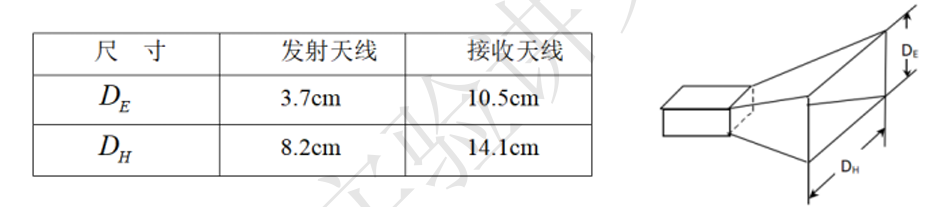
\includegraphics[width=0.7\textwidth]{figures/p01.png}
    \caption{角锥喇叭天线尺寸}
\end{figure}

实验用到的一些概念公式如下：

\subsection{近场和远场}

天线是一种能量转换装置，发射天线将导行波转变为电磁波，接收天线则把电磁波转换为导行波。如图3-3通常根据观察点与天线的距离不同，可将观察点周围的场的区域划分为感应近场区、辐射近场区和辐射远场区。

感应场区的边界条件：$r<\frac{2a^2}{\lambda}$

远场条件：$r\gg\frac{2D_eD_H}{\lambda}$ \quad (m)

\begin{figure}[h]
    \centering
    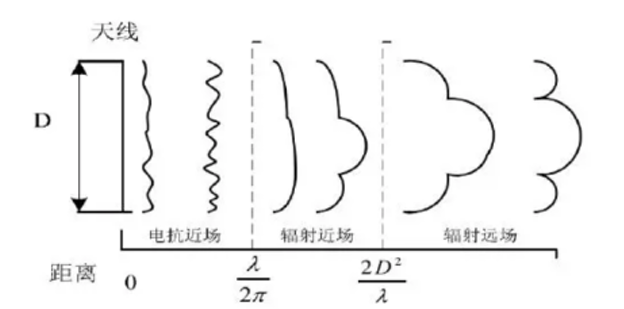
\includegraphics[width=0.7\textwidth]{figures/p02.png}
    \caption{天线场区}
\end{figure}


\subsection{反射系数$\Gamma$，电压驻波比$VSWR$，回波损耗$RL$三者转换关系}

\[
\Gamma = \frac{VSWR-1}{VSWR+1}
\]

\[
RL = 20\log|\Gamma|
\]

\subsection{电磁波在空间传播中与距离的关系（弗里斯传输公式）}

\[
\frac{P_r}{P_t} = \left(\frac{\lambda}{4\pi R}\right)^2 G_t G_r
\]

其中$R$为收、发天线距离（本实验$R$取收发天线喇叭口之间的距离）。

$dBm$与$W$的转换：$dBm = 10\log\left(\frac{W}{1mW}\right), \quad W = 10^{\frac{dBm}{10}} \times 1mW$

$G_t, G_r$是发射、接收天线增益。与$dBi$为单位的增益换算：$G_t(G_r) = 10^{\frac{G_t(G_r)}{10}}$

根据工程经验，实际的增益值比该计算值小3-5dBi。

\subsection{天线增益}

增益是天线极为重要的一个参数，用它可以衡量天线辐射能量的集中程度。短形波导锁电的角锥喇叭天线的增益理论值参见P3“矩形波导锁电角锥喇叭天线理论分析”。

此外， 还可用以下公式估算矩形角锥喇叭天线增益：

\[
G = 0.51 \frac{4\pi A_p}{\lambda^2} \quad (A_p = D_e \times D_H)
\]

在实际工程测试中，天线的增益有多种测试方法。本系统选用的是弗里斯和波束宽度法。

弗里斯法利用上述3-3的弗里斯公式，当发射天线的增益已知或收发天线的增益相同的时候，根据公式即可计算可求解的接收天线的增益。

\[
G_t(dB) + G_r(dB) = \frac{1}{2} \left[20\log \left( \frac{4\pi R}{\lambda}\right) - 10\log \frac{P_c(dB) } {P_t(dB)}\right]
\]

\[
G(dB) = \frac{1}{2}\left[20\log \left( \frac{4\pi R}{\lambda}\right) - (P_c(dB) - P_t(dB))\right]
\]

波束宽度法是通过天线方向图的H面和E面半功率波束宽度，即3dB点的波束宽度从而计算天线增益的方法。

\[
G(dB)=\frac{10lgC}{\theta_{-3A}\theta_{-3E}}
\]

公式中，$\theta_{-3A}$ 和$\theta_{-3E}$分别代表H面和E面方向3dB点波束宽度，单位为角度，C工程上根据经验取值，通常普通天线为32400，反射面天线如卫星电视接受天线为27000，对数周期天线为41000。

\subsection{喇叭天线半功率波束宽}

${H}$面：$2\theta_{0.5}\approx1.18\frac\lambda{D_H}(rad)$

${E}$面：$2\theta_{0.5}\approx0.89\frac\lambda{D_E}(rad)$


\subsection{天线轴向交叉极化隔离度}

$$XPD=P_{cop}(dBm)-P_{xp}(dBm)$$
公式中，$P_{cop}$为同极化信号功率，$P_{xp}$为交叉极化信号功率。
\section{实验设备}

实验装置如图
\begin{figure}[H]
    \centering
    \begin{minipage}[b]{0.5\linewidth}
        \centering
        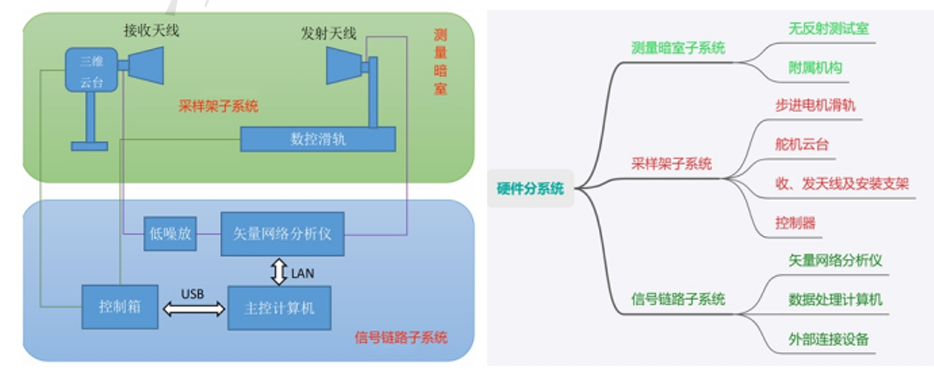
\includegraphics[width=0.9\textwidth]{figures/p03.png}
        \caption{天线测控系统}
        \label{}
    \end{minipage}%
    \begin{minipage}[b]{0.5\linewidth}
        \centering
        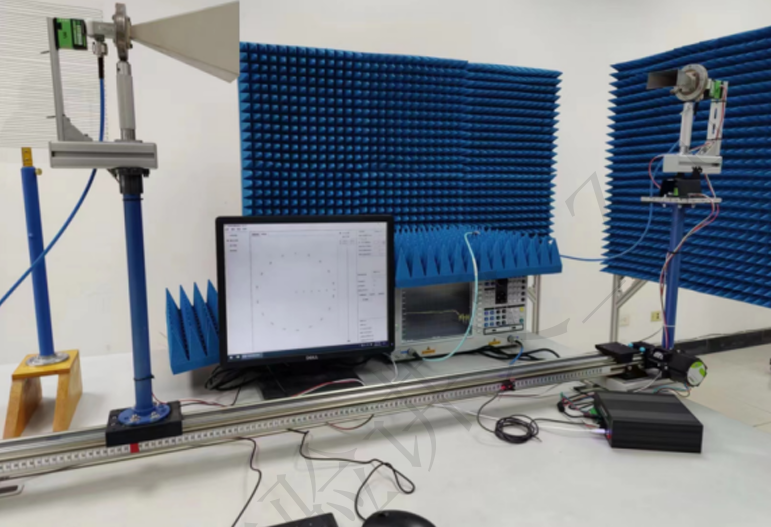
\includegraphics[width=0.9\textwidth]{figures/p04.png}
        \caption{天线测控系统实物图}
        \label{}
    \end{minipage}
\end{figure}
\section{实验内容}
\subsection{实验前准备}

\subsubsection{采样架控制器开机前准备}
天线采样架控制器开机前，必须确保接收天线位于滑轨的光电检测传感器的左侧，此时可手动调整滑轨位置(注意：开机后滑轨和舵机将被锁定，
天线采样架控制器开机前，必须确保接收天线位于滑轨的光电检测传感器的左侧，此时可手动调整滑轨位置(注意：开机后滑轨和舵机将被锁定，
此时不得强制调整以免损伤电机),然后打开控制器电源，接收天线将向发射天线端移动，经过光电传感定位后，最终停在为收发天线间距为零的位置，可记录此时滑轨标尺的位置。
\subsubsection{检查接线，开启电源}
检查计算机与天线采样架控制器的 USB 接口以及和矢量网络分析仪的LNA 口连线是否正常，打开计算机与矢网的电源。

\subsubsection{打开程序并连接}
打开计算机桌面的“天线测量”程序，点击左上角“连接”菜单分别查找并连接天线控制器和网络分析仪。

\subsubsection{数据保存与导出}
接下去就可根据具体的实验内容进行天线特性的测量，在测量过程中请规范操作，实验数据支持导出处理，建议不要保存在 C 盘，以免重启后清空。微波屏蔽板可移动到合适的位置以减少其他电磁波的干扰。

\subsubsection{舵机零位调试}
在测试窗口点击[调试],可调出调试窗口，在此窗口中，可调整发射天线水平方位角度(一号舵机角度校正值),发射天线轴向角度(二号舵机角度校正值),接收天线轴向角度(三号舵机角度校正值)。在天线参量测量前，需要调节收发天线极化方向相同，轴向对准时，通过此处调节。

\begin{figure}[h]
    \centering
    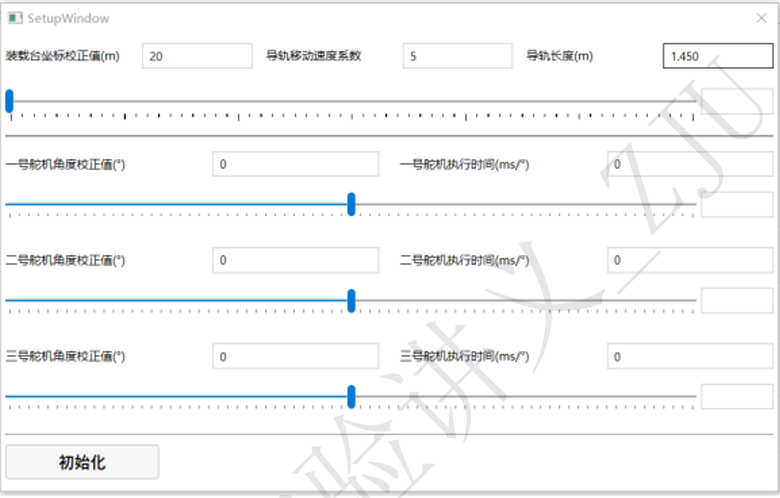
\includegraphics[width=0.7\textwidth]{figures/p05.png}
    \caption{调试界面}
\end{figure}

\subsection{电路特性参数测量}

\subsubsection{驻波比、反射系数、回波损耗测量}

驻波比、反射系数、回波损耗三折的关系可以转换，所以只要测量一个参数就可以计算另外的参数。

实验步骤：在[调试]窗口，调节收、发天线极化方向，轴向角度一致。在测试程序中，如图 3-7,依次选择[S 参数测量]、[驻波比]、[S11](矢网端口 1连接发射天线，端口 2 连接接收天线),确认收发天线的初始状态，设定扫描的起始和终止频率，点击[矢网初始化]、[刷新]之后就可以在测试窗口看到驻波比曲线。观察记录测试结果，并可调整参数重新测试。
\begin{figure}[H]
    \centering
    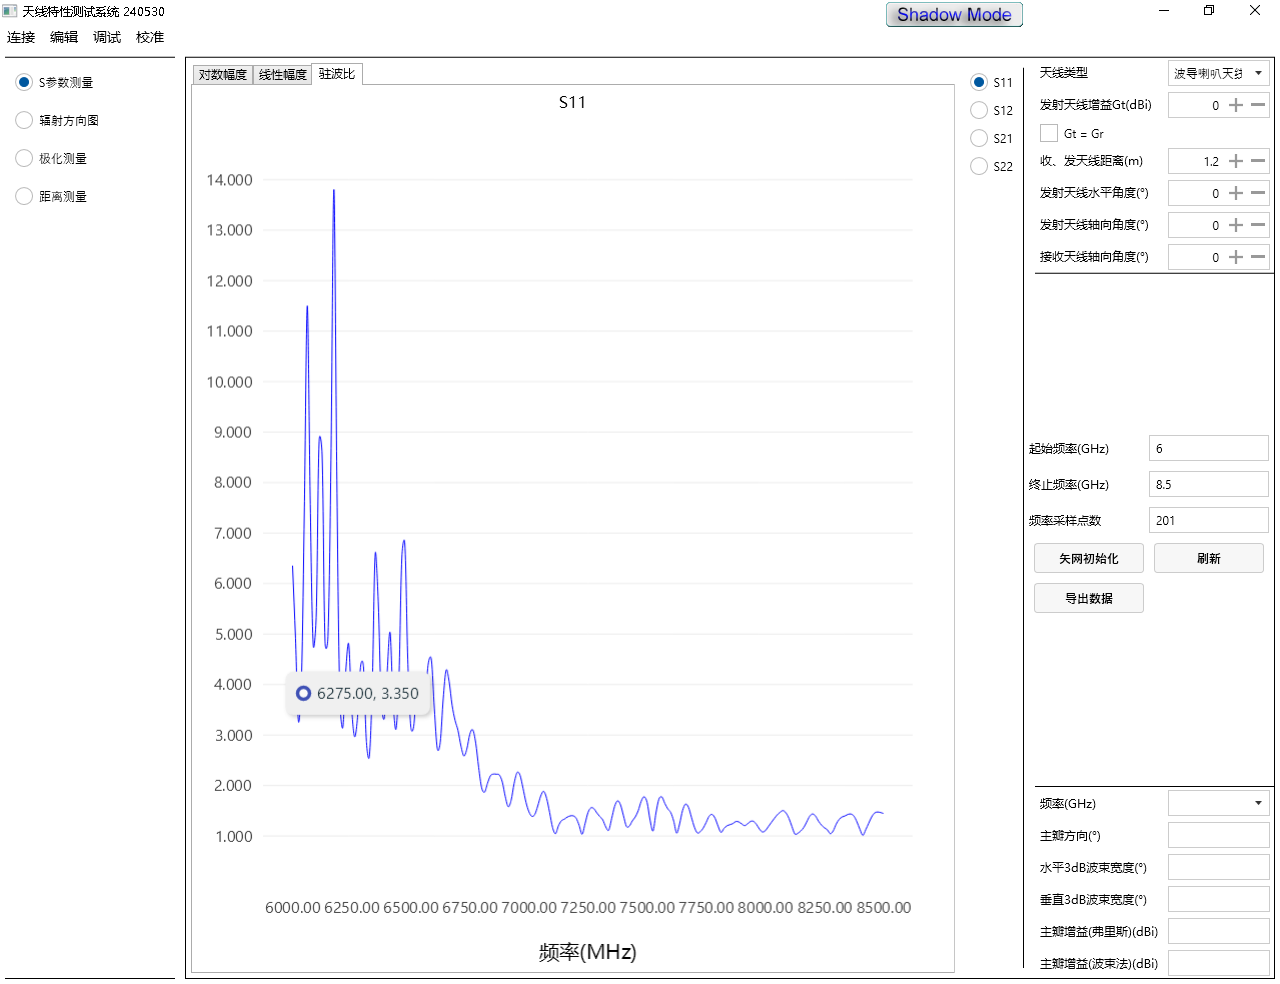
\includegraphics[width=0.7\textwidth]{figures/p11.png}
    \caption{驻波比测量结果}
\end{figure}

\subsubsection{扫频测量}

实验步骤：在[调试]窗口，调节收、发天线极化方向，轴向角度一致。在测试程序中，如图 3-8,依次选择[S 参数测量]、[对数幅度]、[S21],确认收发天线的初始状态，设定扫描的起始和终止频率，点击[矢网初始化]、[刷新]之后就可以在测试窗口看到天线的扫频曲线。观察记录测试结果，并可调整参数重新测试。

\begin{figure}[H]
    \centering
    \begin{minipage}[b]{0.5\linewidth}
        \centering
        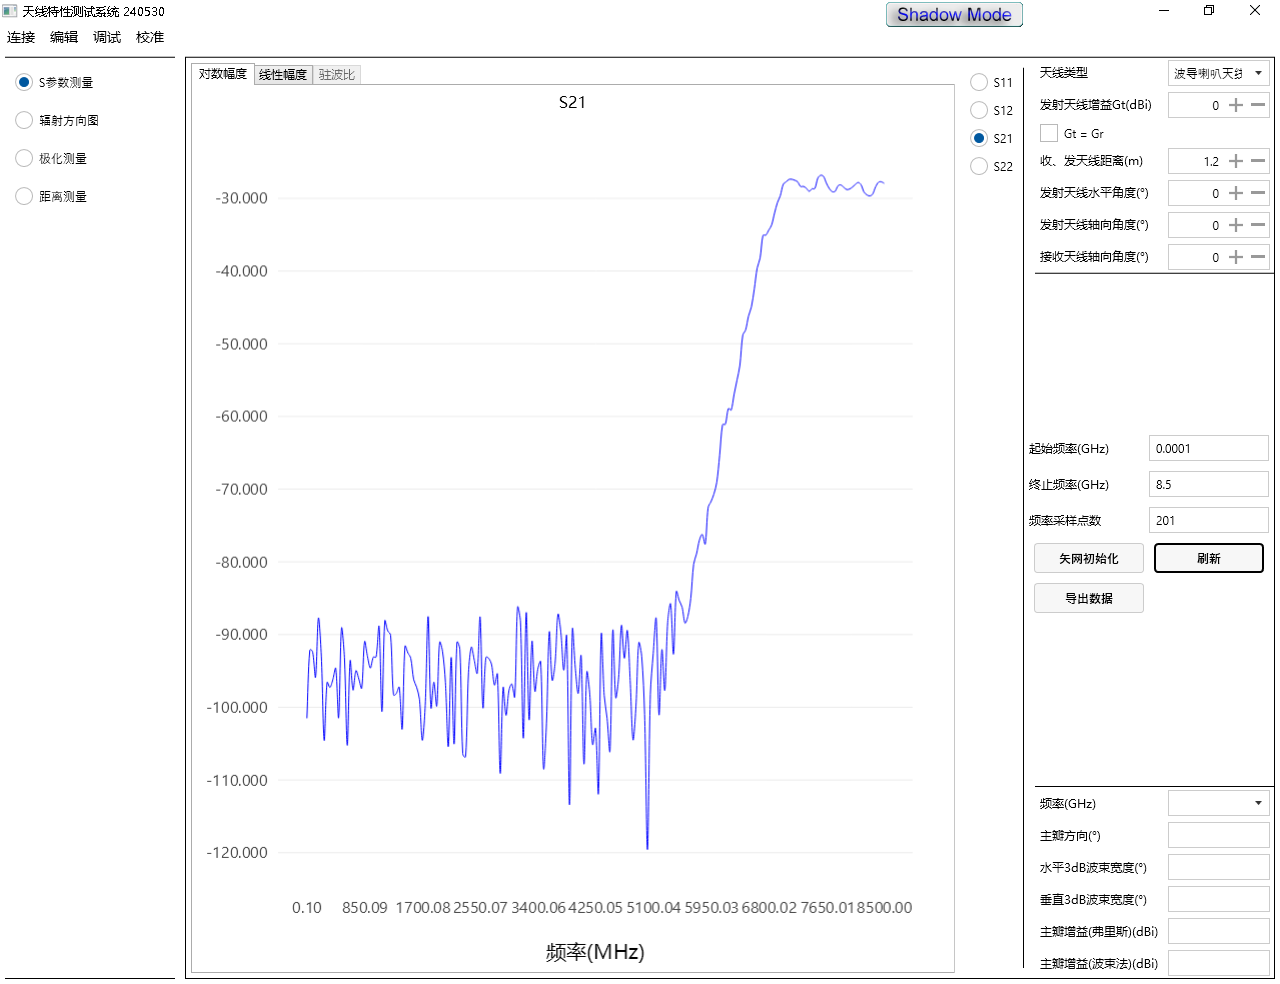
\includegraphics[width=0.95\textwidth]{figures/p21.png}
        \caption{天线扫频测量}
        \label{}
    \end{minipage}%
    \begin{minipage}[b]{0.5\linewidth}
        \centering
        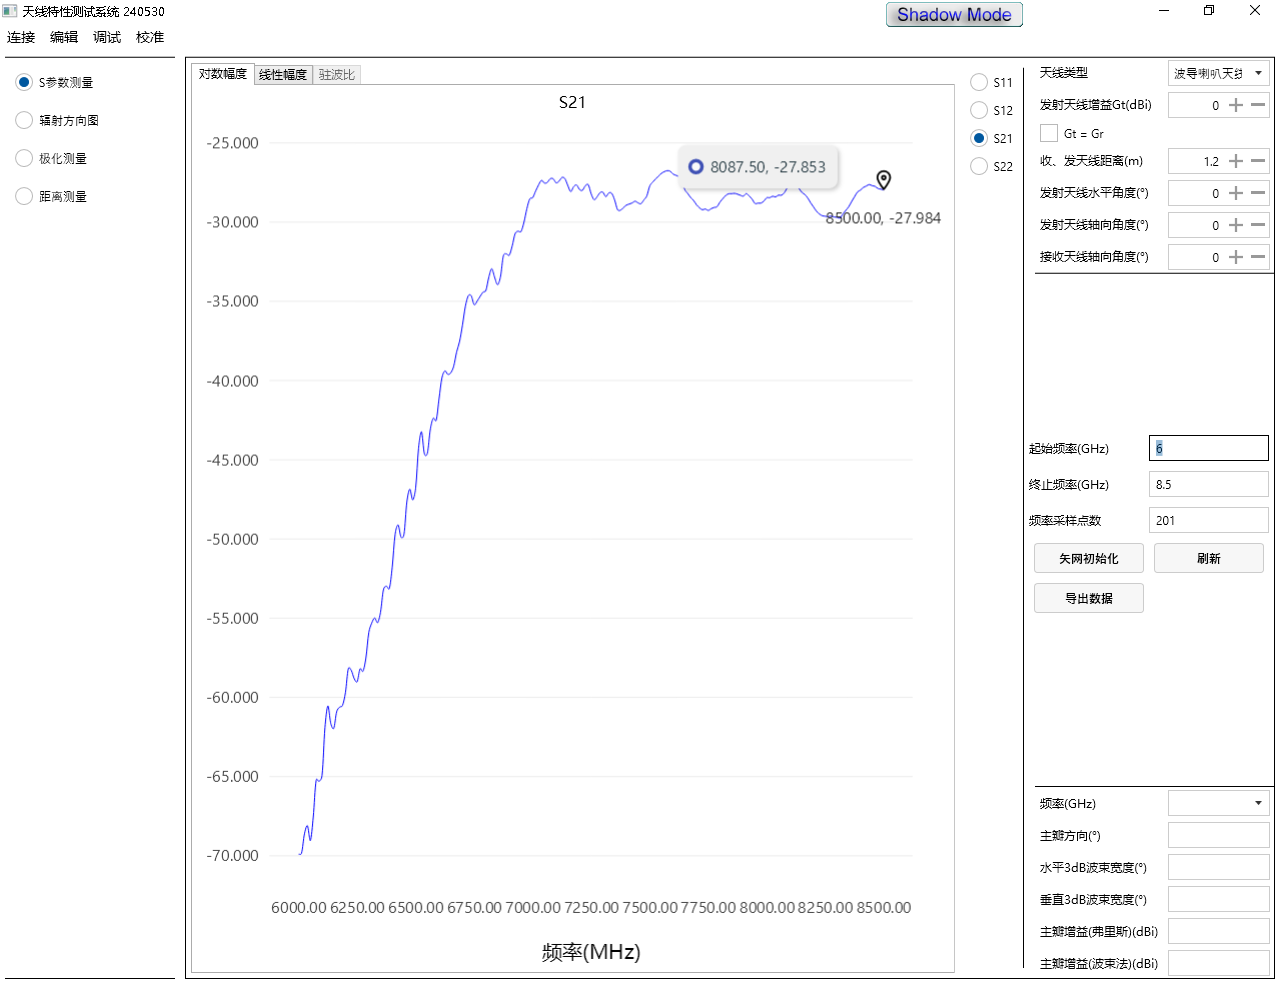
\includegraphics[width=0.95\textwidth]{figures/p22.png}
        \caption{天线扫频测量放大图}
        \label{}
    \end{minipage}
\end{figure}

\subsection{喇叭天线辐射方向图测量}
天线方向图表征天线在空间中各个方向上所具有的发射或接收电磁波的能力，是天线辐射特性的重要参数。完整的方向图是一个三维空间图，实际工程中通常只需测量水平面 H 方向图和垂直面 E 方向图。

实验步骤：在[调试]窗口，调节收、发天线极化方向，轴向角度一致。

\subsubsection{水平面方向图测量}
在测试程序中，如图 3-9,依次选择[辐射方向图]、 [极坐标]、[水平方向图],右侧框图中，天线类型选择“波导喇叭天线”,发射天线增益未知则默认为 0dBi, 当发射与接收天线相同的时候可勾选两者增益相同，设置收发天线间的距离(注意：收发天线间的距离指的是两个喇叭口之向的问题，可根据滑轨侧边的标尺来读取)。发射天线水平角度、发射和接收天线的极化角度无需设置(测试开始后都将转到0°的位置),测试频率可以设置多个，填入数据后回车即可(建议根据之前驻波比测量结果，选择三个频率进行测量)。开始、结束角度和采样步进选择默认值。点击[矢网初始化]、[开始测试之后，发射天线将转到水平方位开始角度，并以步进值向结束角度旋转， 同时在方向图窗口实时显示测试曲线。测试过程中注意人员不要遮挡天线，并可移动屏蔽板防止其他十扰信号，等待测试完成后，观察测试结果可导出数据， 如有明显偏差可调整参数重新测试。
\begin{figure}[H]
        \centering
        \subcaptionbox{水平面方向图测量6GHz}[0.33\textwidth][c]{
            \centering
            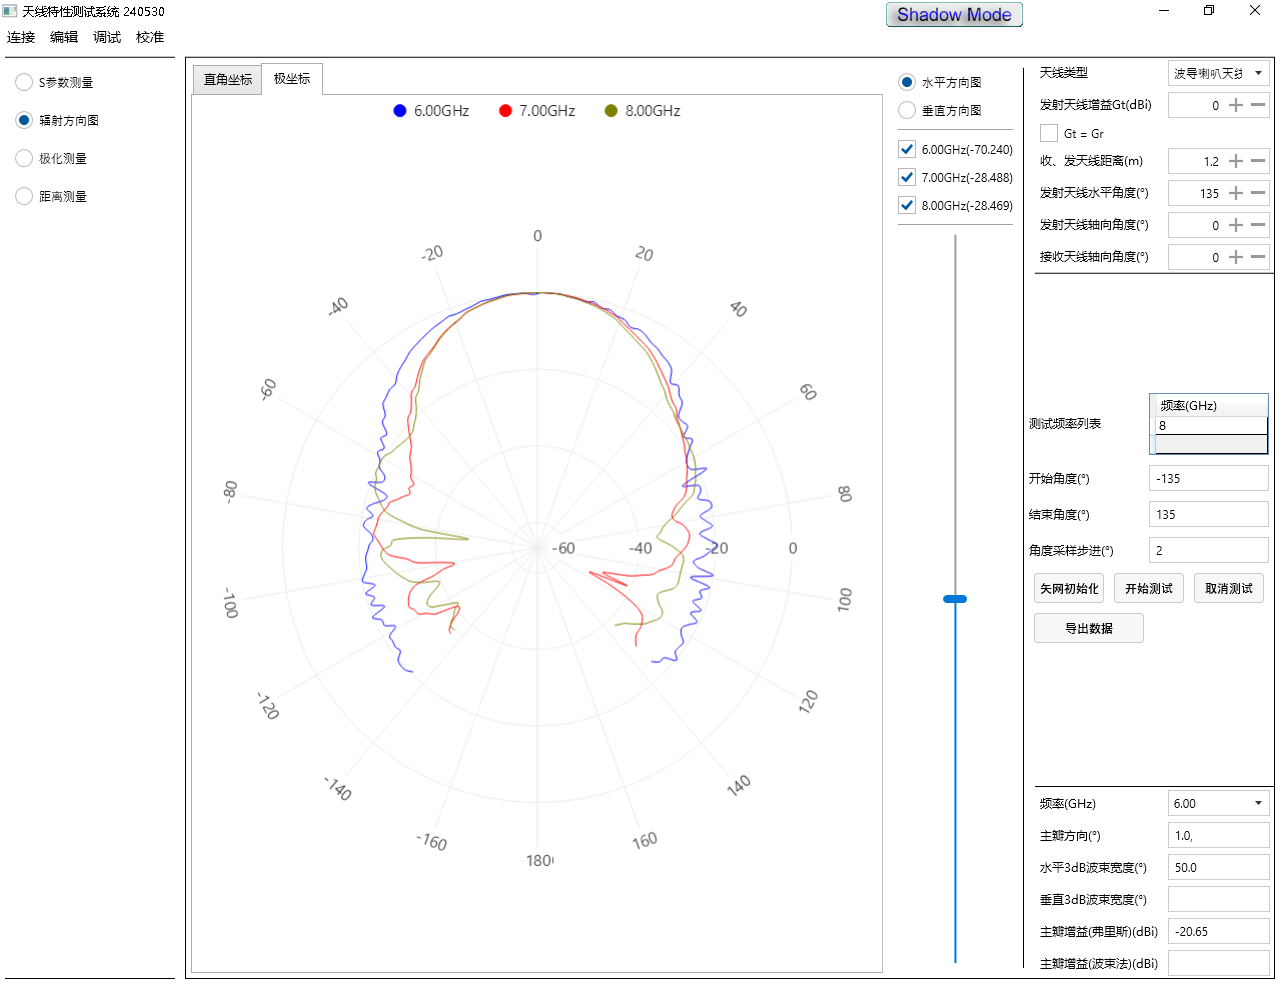
\includegraphics[width=0.32\textwidth]{figures/p31.png}
            \label{}
        }%
            \subcaptionbox{水平面方向图测量7GHz}[0.33\textwidth][c]{
            \centering
            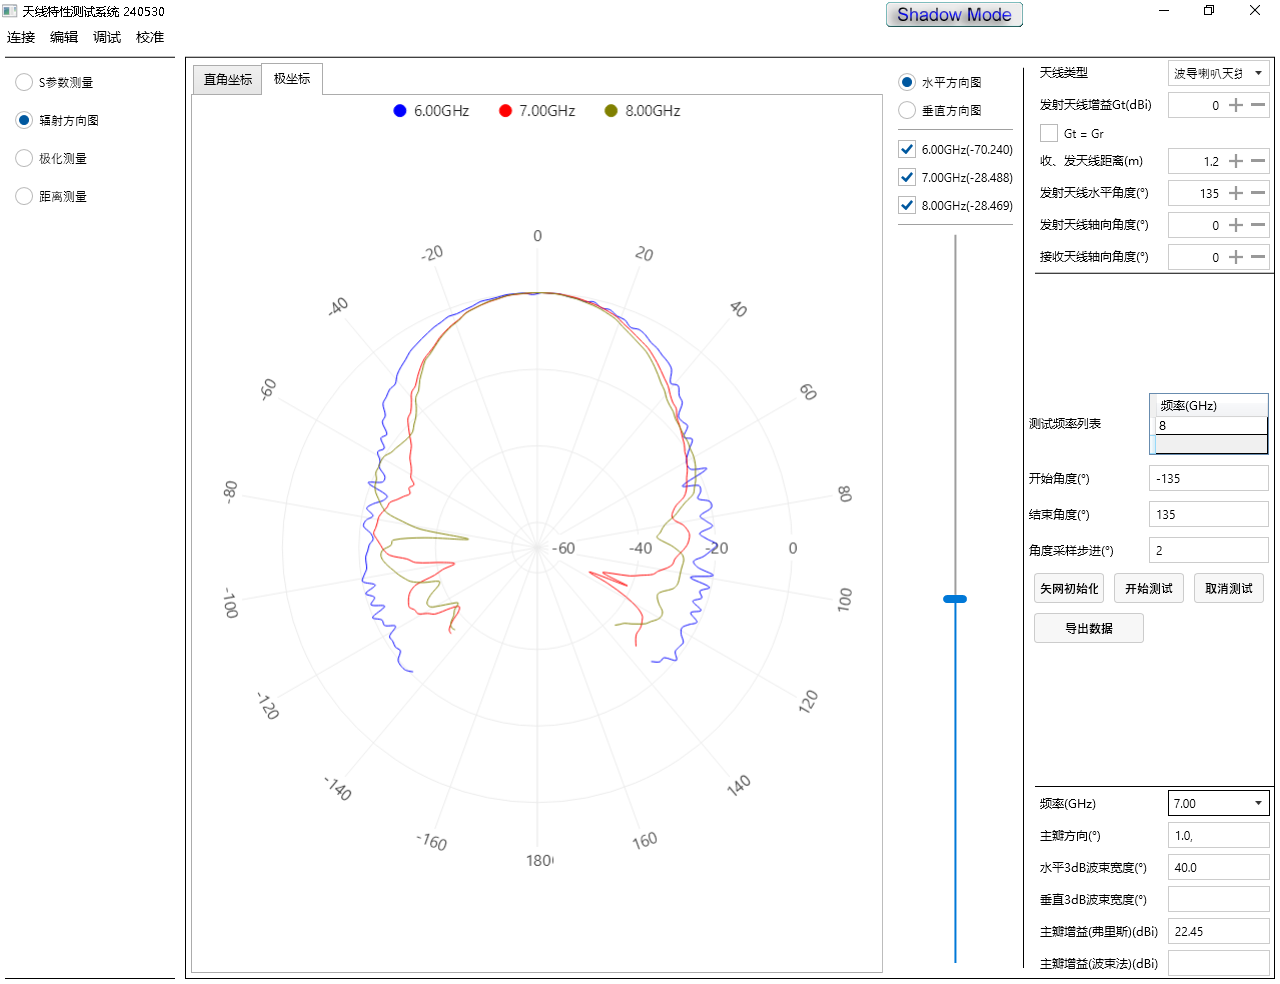
\includegraphics[width=0.32\textwidth]{figures/p32.png}
            \label{}
        }%
            \subcaptionbox{水平面方向图测量8GHz}[0.33\textwidth][c]{
            \centering
            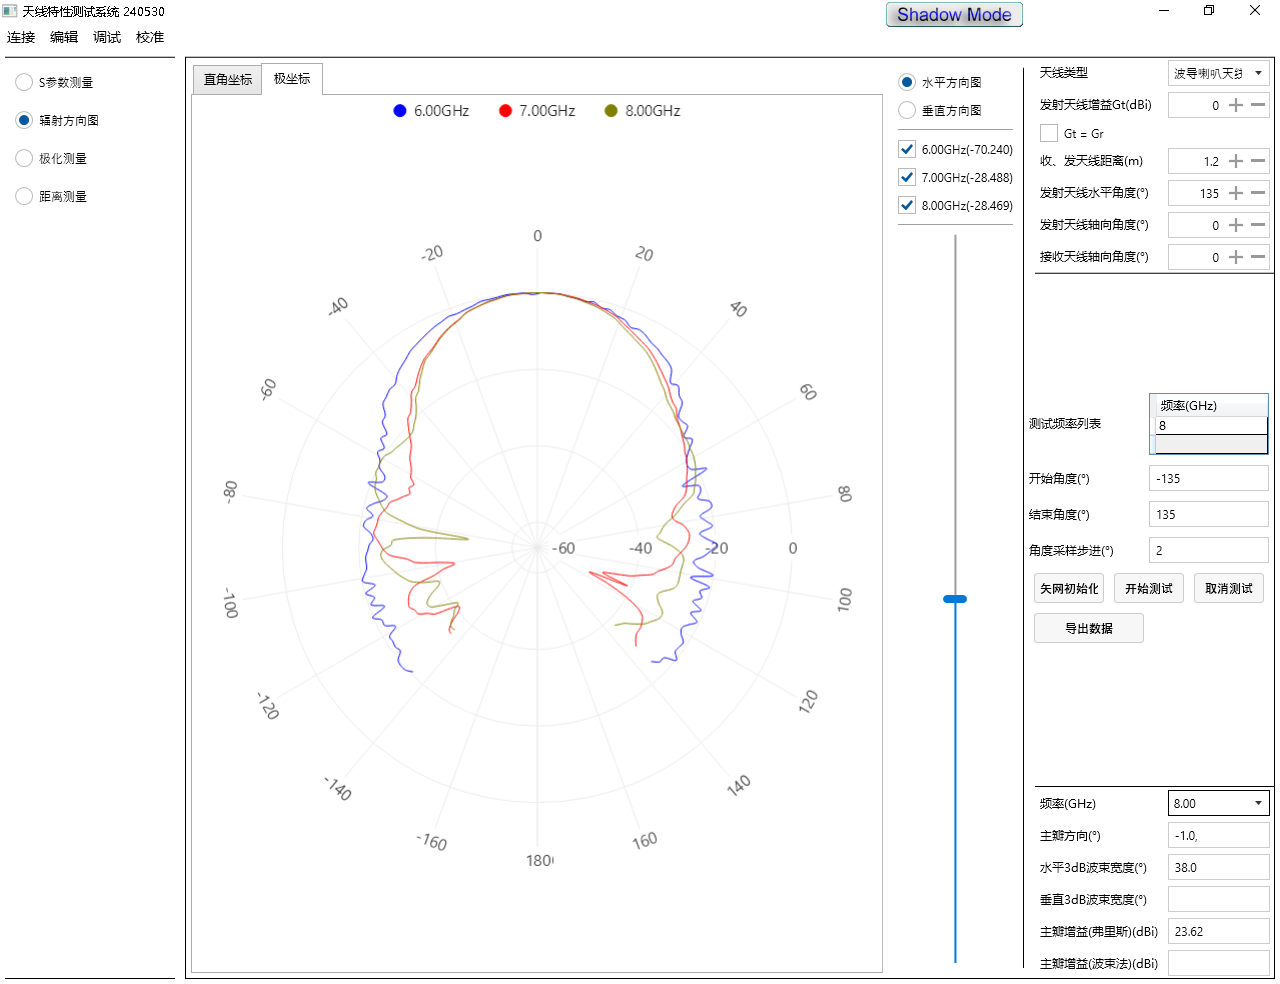
\includegraphics[width=0.32\textwidth]{figures/p33.png}
            \label{}
        }%
        \label{}
\end{figure}

\subsubsection{垂直面方向图测量}
在测试程序中，依次选择[辐射方向图]、[极坐标]、 [垂直方向图],可设置收发天线间的距离，开始、结束角度和采样步进。发射天线水平角度、发射和按收天线的极化角度无需设置(测试开始后都将转到到0和 90°的位置),其他设置和水平方向图测试相同，等待测试完成后，观察测试结果可导出数据，如有明显偏差可调整参数重新测试。天线方向图测试完成后，在程序右下角将自动显示主瓣，3dB 点波束宽度、增益等计算值。
\begin{figure}[H]
        \centering
        \subcaptionbox{垂直面方向图测量6GHz}[0.33\textwidth][c]{
            \centering
            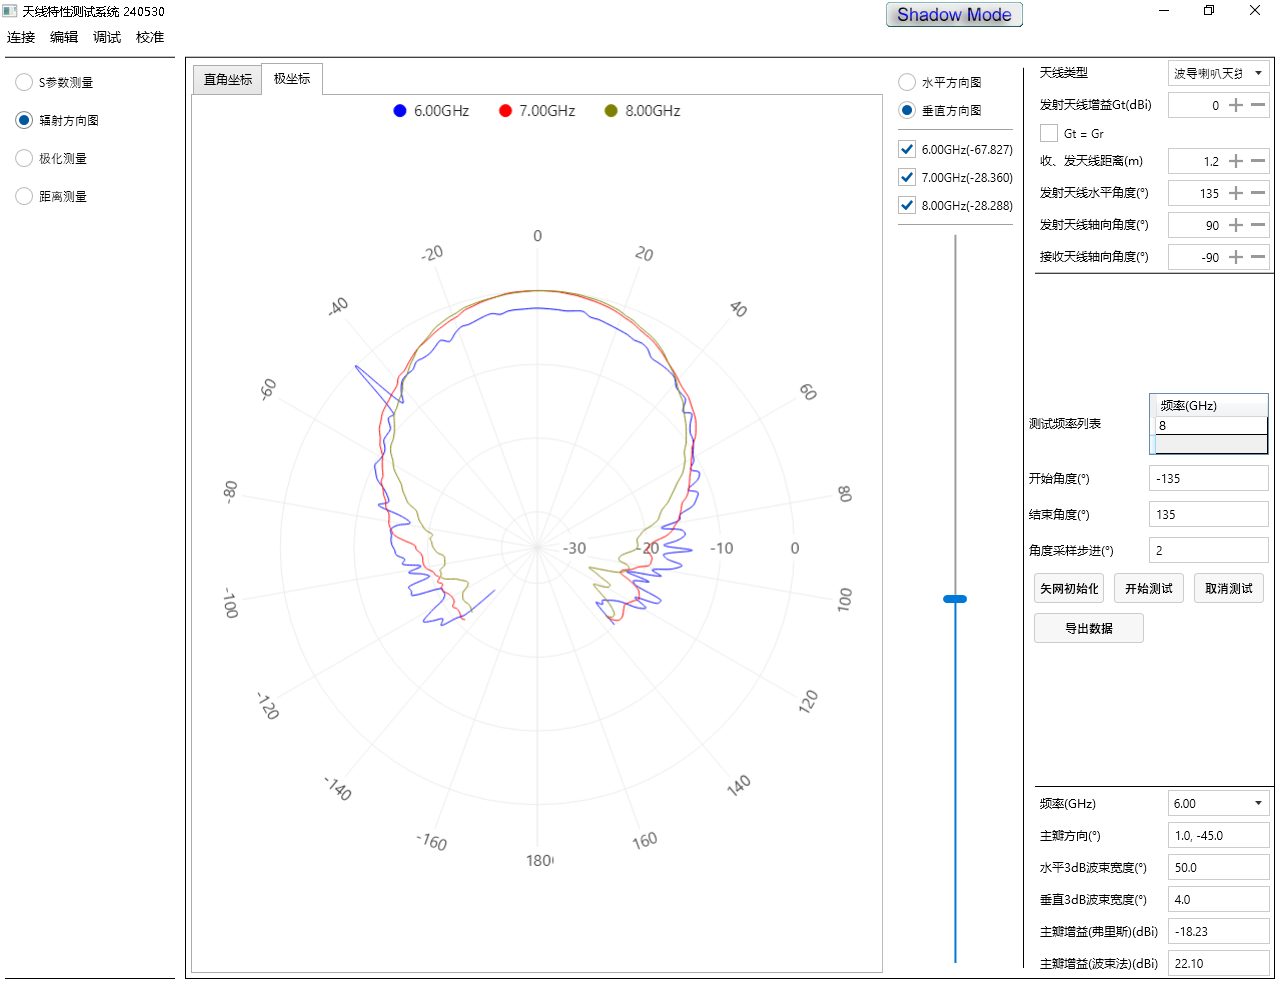
\includegraphics[width=0.32\textwidth]{figures/p34.png}
            \label{}
        }%
        \subcaptionbox{垂直面方向图测量7GHz}[0.33\textwidth][c]{
            \centering
            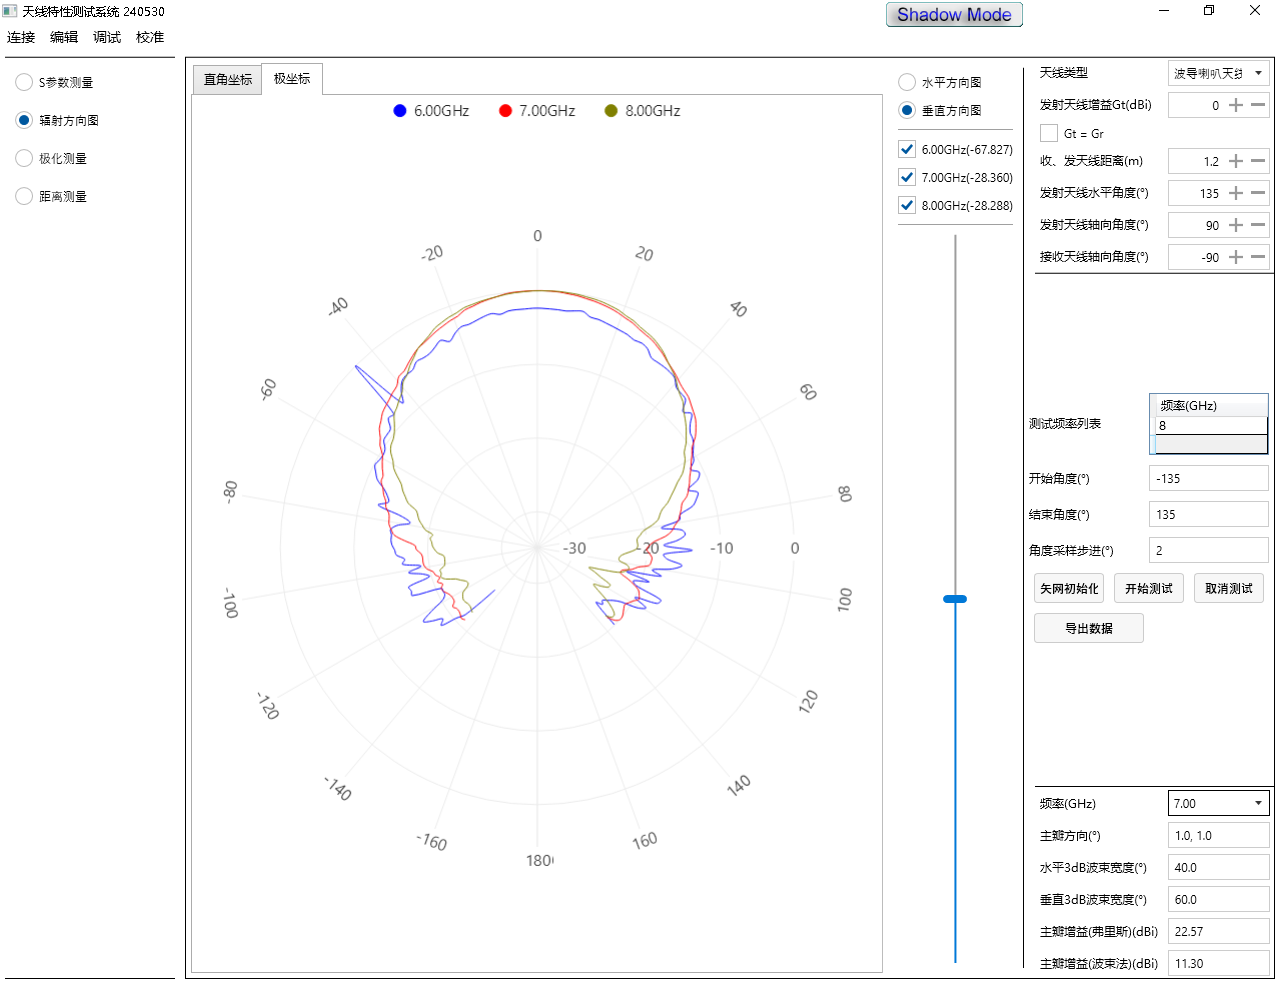
\includegraphics[width=0.32\textwidth]{figures/p35.png}
            \label{}
        }%
        \subcaptionbox{垂直面方向图测量8GHz}[0.33\textwidth][c]{
            \centering
            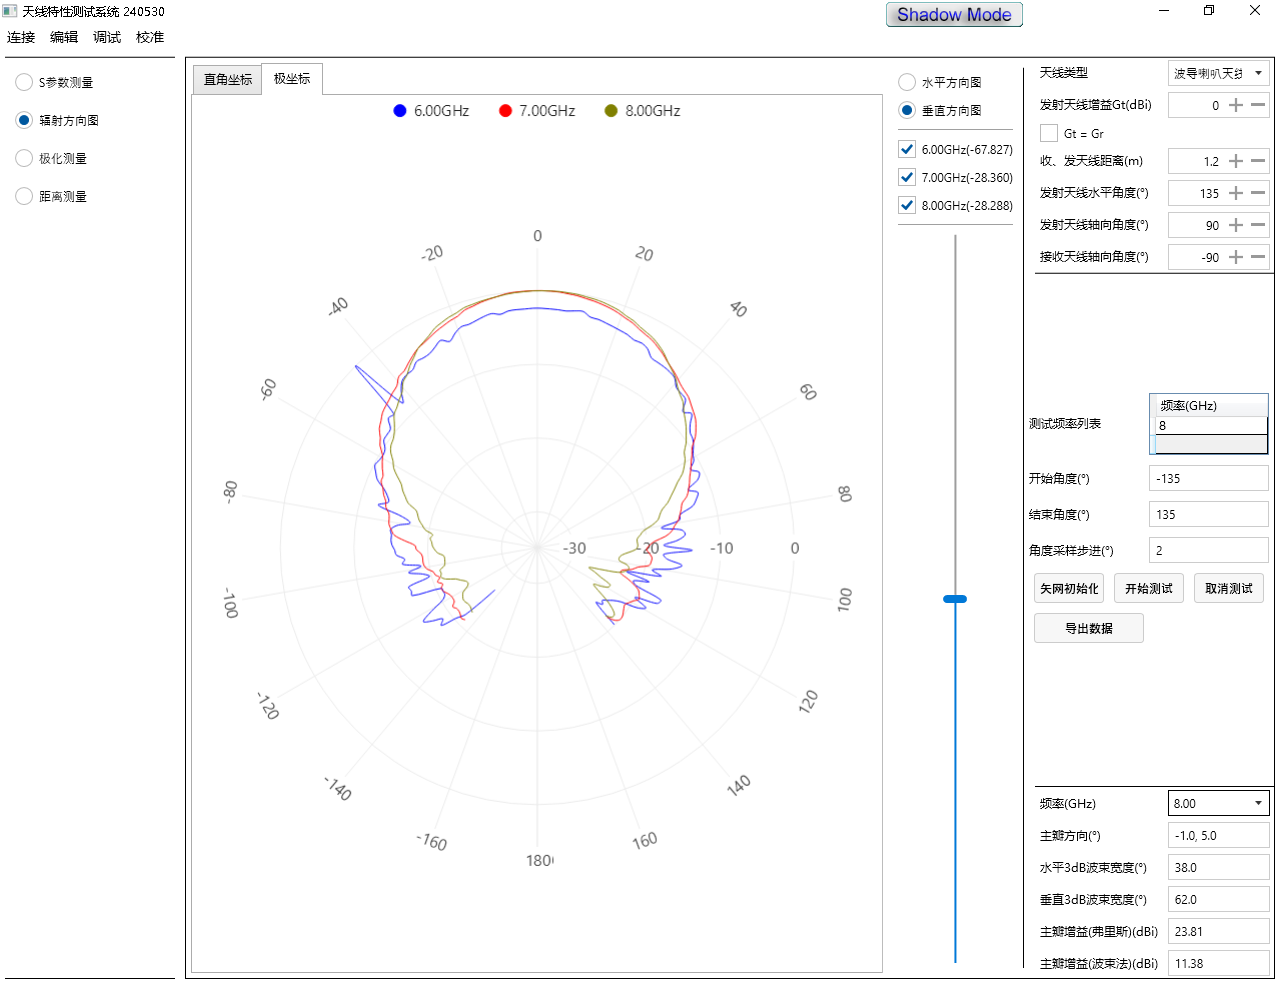
\includegraphics[width=0.32\textwidth]{figures/p36.png}
            \label{}
        }%
        \label{}
\end{figure}

\subsection{极化测量}

实验步骤：在[调试]窗口，调节收、发天线极化方向，轴向角度一致。

\subsubsection{天线极化测量}
在测试程序中，依次选择[极化测量]、[对数幅度]「常规极化测量],确认收发天线的初始状态，设定测试频率，常规极化测试时发射天线极化角度默认从0°扫描到90°,点击[矢网初始化]、[开始]之后就可以在测试窗口看到天线的极化测试曲线。观察记录测试结果，并可调整

\begin{figure}[H]
    \centering
    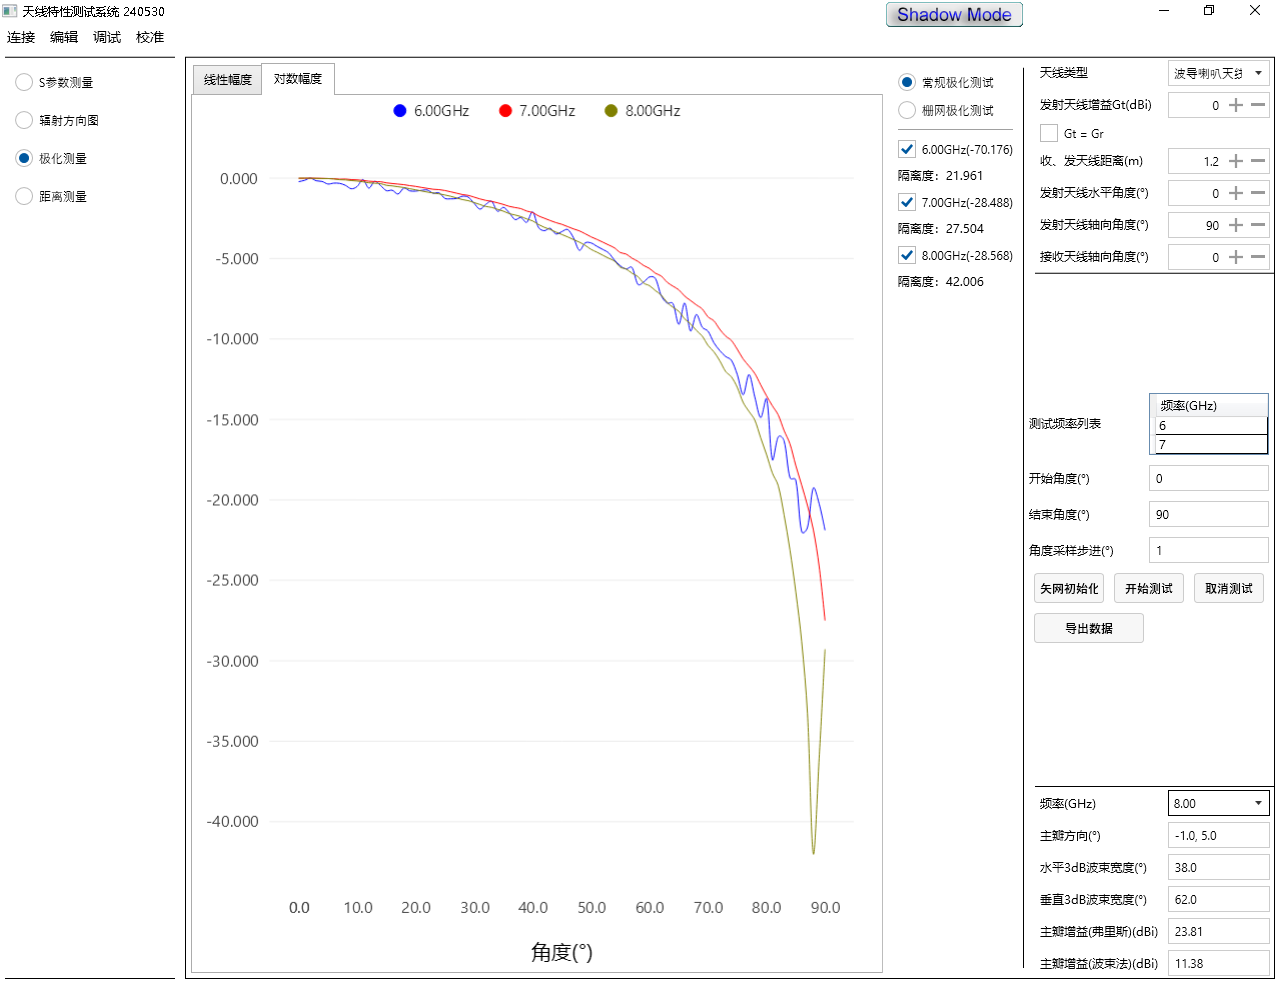
\includegraphics[width=0.9\textwidth]{figures/p41.png}
    \caption{常规极化测试}
\end{figure}

\subsubsection{极化栅网特性测量}
极化栅网是在一块玻璃上间隔均匀的缝隙拉上金属丝，如果金属丝的宽度与缝隙的宽度都比波长小得多，则对于投射到栅网上的电磁波，对于电场平行于缝隙方向的电磁波将被全反射，而垂直于缝隙方向的电磁波将能顺利通过。所以将极化栅网放到发射天线前面，则按收天线所按收到的信号大小随着极化栅网旋转角度的改变而改变。极化栅网特性测量时，将一个水平栅网放置在收发天线之间，在测试程序中，除选择[栅网极化测量]外，其他设置和“天线极化测量”相同。测试过程中，收、发天线将从
$0^{\circ}$到90°轴向相对旋转，以实现和极化栅网旋转同等的效果。设置完成后，
点击[矢网初始化]、[开始]之后就可以在测试窗口看到天线的极化测试曲线。观察记录测试结果，并可调整参数重新测试。

\begin{figure}[H]
    \centering
    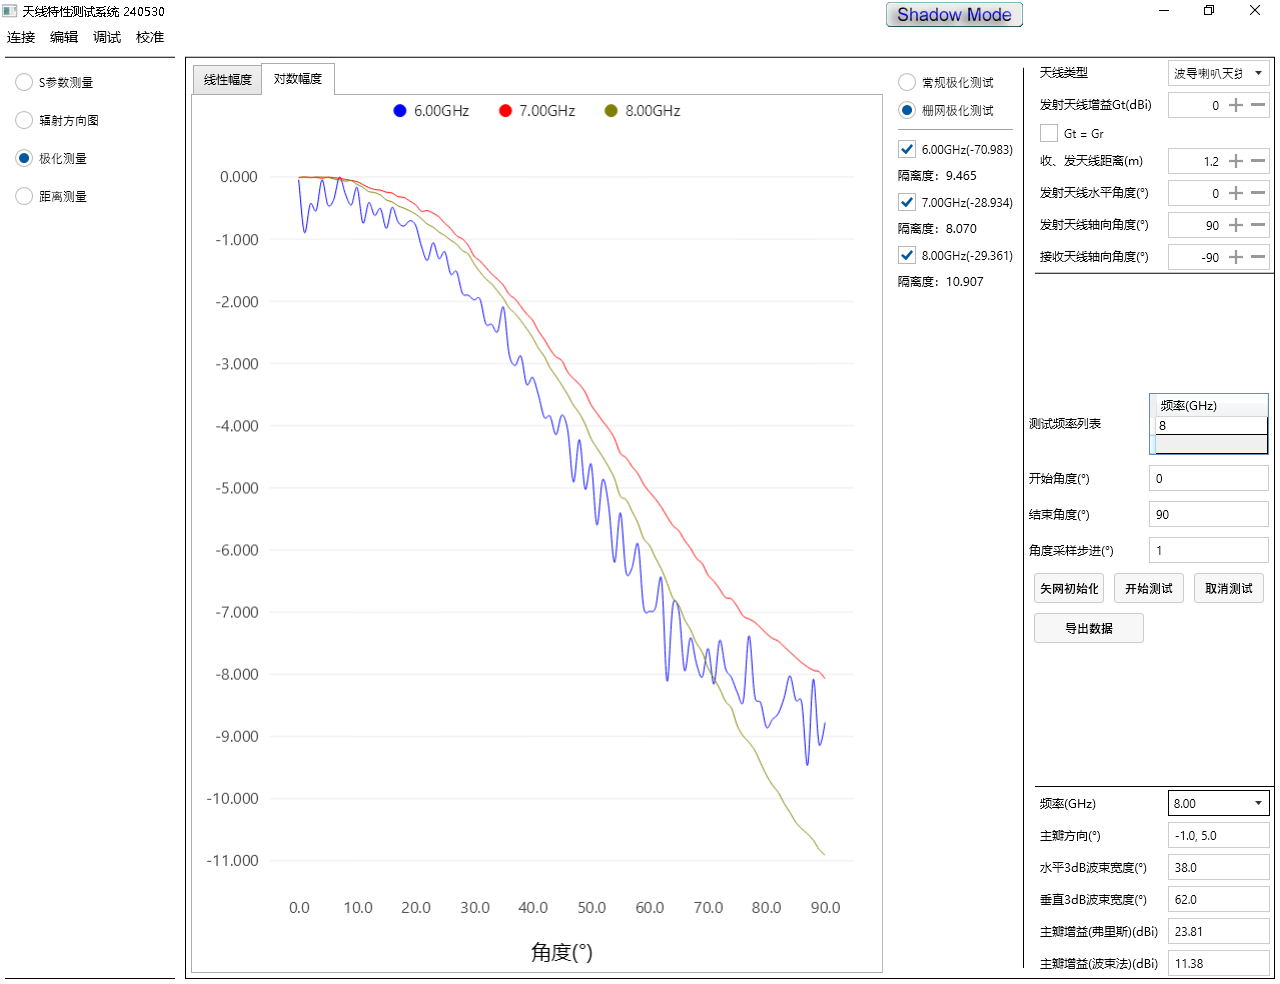
\includegraphics[width=0.73\textwidth]{figures/p42.png}
    \caption{栅网极化测试}
\end{figure}

\subsection{电磁波在空间传播中与距离的关系测量}

实验步骤：在测试程序中，如图 3-12.依次选择[距离测量][对数幅度]确认收发天线的初始状态，
设定测试频率、发射天线在滑轨上的的起始位置、 结束位置、采样步进等参数，点击[矢网初始化]、[开始]之后就可以在测试窗口看到电波在空间传播时按收到的信号与距离的关系曲线。观察记录测试结果并可调整参数重新测试。

\begin{figure}[H]
    \centering
    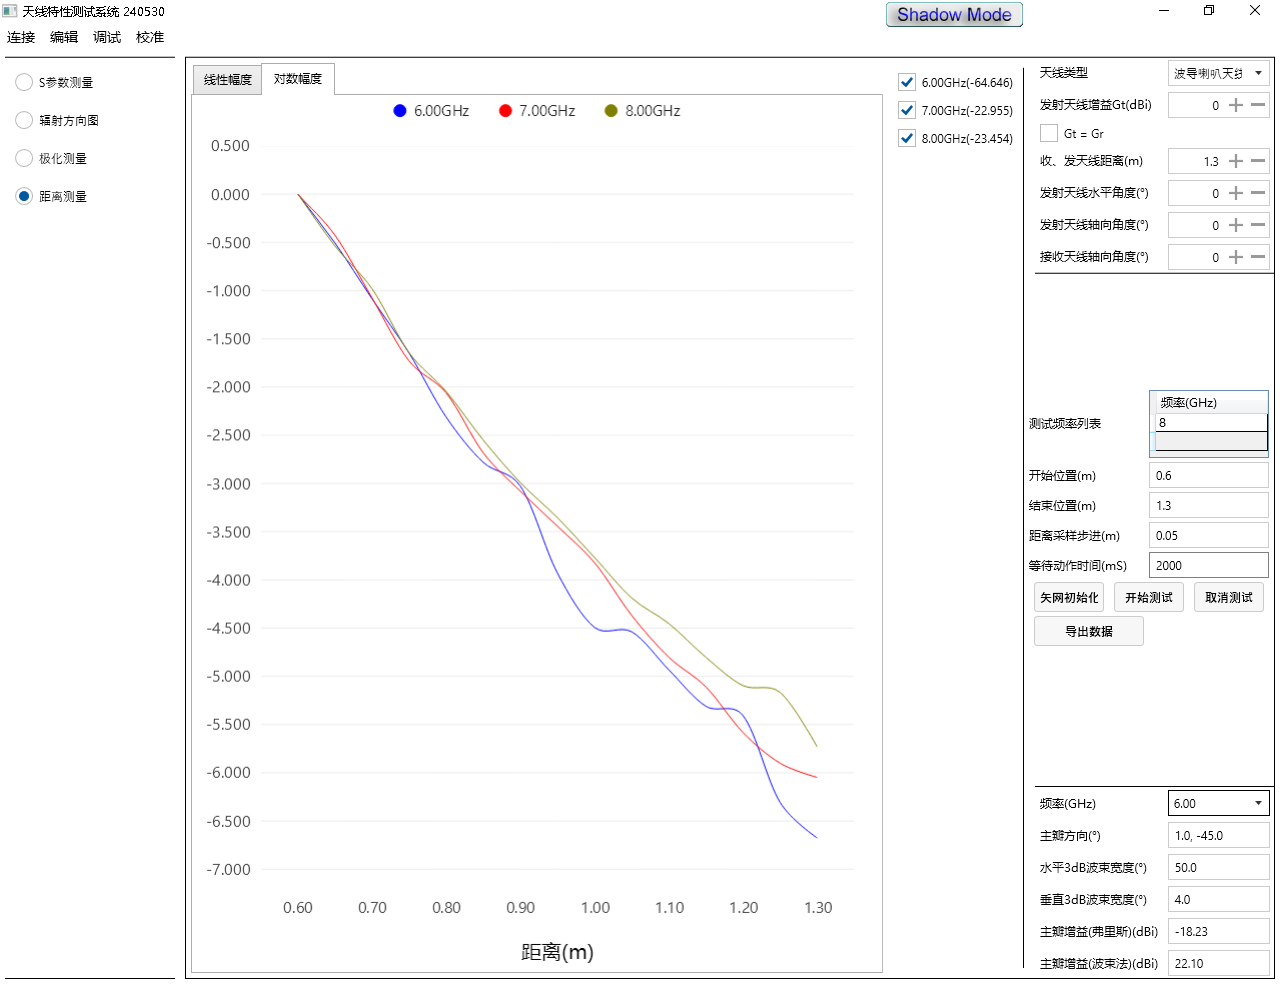
\includegraphics[width=0.73\textwidth]{figures/p51.png}
    \caption{空间传播中与距离关系测量}
\end{figure}

\section{数据分析}

\subsection{天线驻波比测量，存在哪些误差？要提高测量的准确性，需怎么做？}

在天线驻波比测量过程中，存在以下几种误差：

\begin{itemize}
    \item \textbf{仪器精度误差：}矢量网络分析仪的精度会影响测量结果，校准不准确或仪器本身存在精度限制会导致测量数据不准确。
    \item \textbf{连接器和电缆误差：}损坏或质量不佳的连接器和电缆会引入额外的反射和损耗，影响测量准确性。实验中使用的N型转SMA转接头也可能引入无法消除的误差。
    \item \textbf{环境干扰：}外界电磁波（如电磁噪声、其他设备的反射）可能会对测量结果造成干扰。实验中会使用微波屏蔽板来减少这些干扰。
    \item \textbf{天线安装和对准误差：}收发天线的极化方向和轴向对准如果不正确，会导致测量误差。
\end{itemize}

为了提高测量的准确性，可以采取以下措施：

\begin{itemize}
    \item \textbf{精确校准：}每次测量前对矢量网络分析仪进行准确校准，以消除系统误差。
    \item \textbf{高质量组件：}使用特性良好、匹配的连接器和电缆。
    \item \textbf{减少环境干扰：}在电磁屏蔽较好的环境中进行测量，并合理使用微波屏蔽板。
    \item \textbf{精确对准：}仔细调节收发天线的极化方向和轴向，确保其一致和对准。
    \item \textbf{稳定仪器：}确保仪器预热稳定后再进行测量。
\end{itemize}

\subsection{根据导出的数据作出电磁波传播与距离的关系曲线。该曲线接近$\frac1R$,$\frac1{R^2}$还是$\frac1{R^3}$关系？}
\begin{figure}[H]
    \centering
    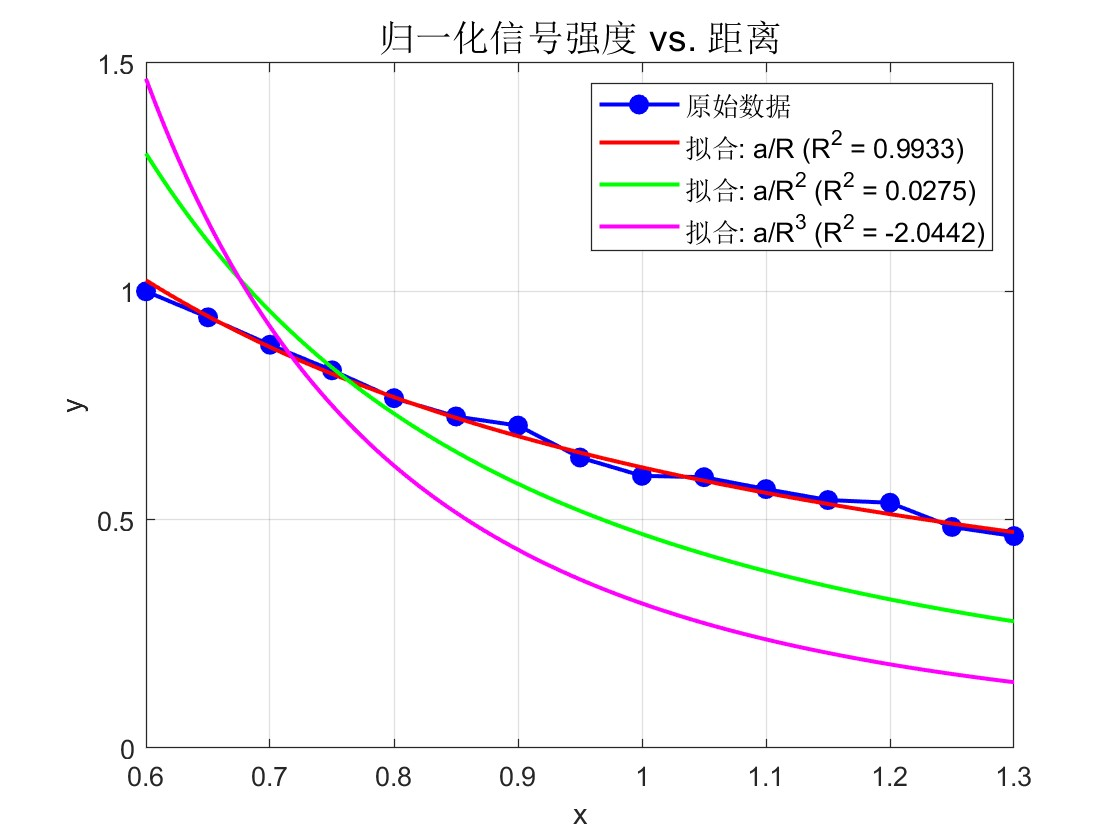
\includegraphics[width=0.73\textwidth]{figures/Matlab1.jpg}
    \caption{电磁波传播与距离关系曲线}
\end{figure}

根据弗里斯传输公式（式3-3）：
\[
\frac{P_r}{P_t} = \left(\frac{\lambda}{4\pi R}\right)^2 G_t G_r
\]

可以看出接收功率$P_r \propto \frac{1}{R^2}$。

实验数据绘制的\textbf{归一化信号强度}(即$\sqrt{P_r})$与$R$关系曲线来看，它接近于$\frac{1}{R}$关系，说明$P_r$与$R$关系曲线接近于$\frac{1}{R^2}$关系，这符合理论预期。电磁波在自由空间传播时，功率密度与距离平方成反比，即遵循平方反比定律。

\subsection{根据数据作出发射喇叭天线极化曲线，横坐标为天线极化角度$\theta$。}

\begin{figure}[H]
    \centering
    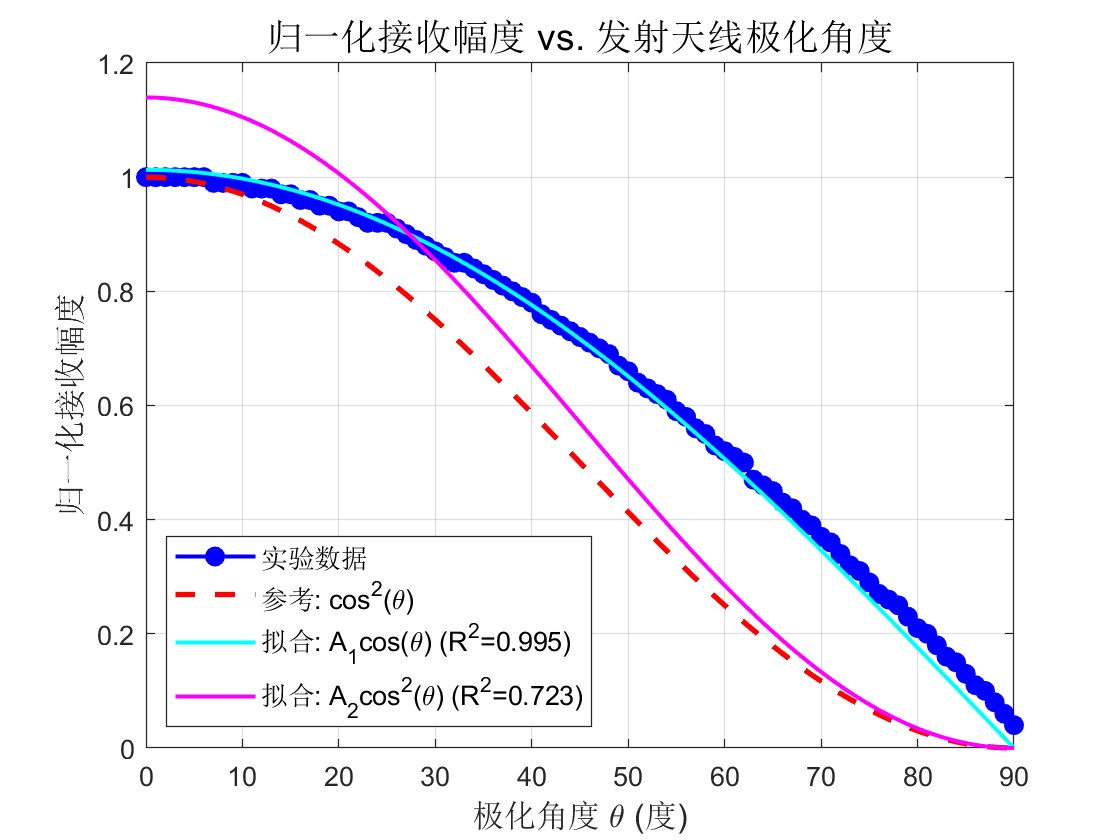
\includegraphics[width=0.73\textwidth]{figures/Matlab2.jpg}
    \caption{喇叭天线极化特性曲线}
\end{figure}


\subsection{从发射喇叭天线极化特性曲线看，接收喇叭天线所接收到的信号与发射
喇叭天线极化角度$\theta$的关系是符合$cos\theta$还是$cos^2\theta$关系？
}

实验数据绘制的\textbf{归一化接受幅度}(即$\sqrt{P_r})$与$\theta$关系曲线来看，
它接近于$cos\theta$关系，说明$P_r$与$R$关系曲线接近于$cos^{2}\theta$关系,
这符合电磁波理论中的极化匹配因子公式：$P_r = P_{max}\cos^2\theta$，其中$P_{max}$是完全极化匹配时的接收功率。

\subsection{如果发射喇叭天线和接收喇叭天线的极化角相差 90°,而极化栅网相对
于发射喇叭天线的极化角度为 45°,极化器对系统的影响如何？}

当发射天线与接收天线极化角相差$90^\circ$时（交叉极化），理想情况下接收天线接收不到信号，因为$P_r = P_{max}\cos^2(90^\circ) = 0$。

当引入一个相对于发射天线极化角度为$45^\circ$的极化栅网时：

由于极化栅网的特性是允许垂直于金属丝方向的电场通过（即平行于缝隙方向），故入射波经过栅网后，极化方向变为$45^\circ$
由于接收天线（与发射天线相差$90^\circ$）与经过栅网后的波极化方向形成$45^\circ$角，此时接收功率为：$P_r = P_{max}\cos^2(45^\circ) = 0.5P_{max}$

结论：极化栅网使接收功率从理论上的0提升至最大可能接收功率的50\%，起到了极化转换的作用。

\subsection{对发射天线计算远区场距离，实验中是否符合远区场条件？}

由远区场条件：
\[
r \gg \frac{2D_HD_E}{\lambda}
\]

根据实验所用的发射天线尺寸：$D_H = 8.2\text{cm}$, $D_E = 3.7\text{cm}$。
在频率$f = 8\text{GHz}$下，波长$\lambda = \frac{c}{f} = \frac{3\times10^8}{8\times10^9} = 3.75\text{cm}$。

计算最小远场距离：
\[
r_{min} = \frac{2 \times 0.082 \times 0.037}{0.0375} \approx 0.162\text{ m} = 16.2\text{ cm}
\]

在实验中，滑轨标尺距离$R = 120cm \gg 20.2\text{cm}$，实验条件基本能视作满足远区场测量条件。

\subsection{分别计算收、发天线理论增益，半功率波束宽度(假定$k\approx1$)。有什么结论？}

\subsubsection{发射天线}

理论增益：
\[
G = 0.51 \frac{4\pi A_p}{\lambda^2}, \quad A_p = D_H \times D_E = 0.003034\text{ m}^2
\]
\[
G = 0.51 \times \frac{4\pi \times 0.003034}{(0.03)^2} \approx 21.59
\]

半功率波束宽度（$k \approx 1$）：
\[
\text{H面}: 2\theta_{0.5H} \approx 1.18\frac{\lambda}{D_H} \approx 24.7^\circ
\quad \text{E面}: 2\theta_{0.5E} \approx 0.89\frac{\lambda}{D_E} \approx 41.3^\circ
\]

\subsubsection{接收天线}
理论增益：

\[
G = 0.51 \frac{4\pi A_p}{\lambda^2}, \quad A_p = D_H \times D_E = 0.014805\text{ m}^2
\]
\[
G = 0.51 \times \frac{4\pi \times 0.014805}{(0.03)^2} \approx 105.4
\]

半功率波束宽度（$k \approx 1$）：

\[
\text{H面}: 2\theta_{0.5H} \approx 1.18\frac{\lambda}{D_H} \approx 14.4^\circ
\quad \text{E面}: 2\theta_{0.5E} \approx 0.89\frac{\lambda}{D_E} \approx 14.6^\circ
\]
【结论】：
大喇叭天线的增益显著高于小喇叭天线，同时波束宽度更窄，方向性更强。这符合天线理论中孔径尺寸与增益和波束宽度的关系：孔径越大，增益越高，波束越窄。

\subsection{当收发天线相同时，可以用什么方法便捷测量天线增益，思考测量时如何消除误差？}

当收发天线相同时($G_t = G_r = G$)，可以使用弗里斯公式法便捷测量天线增益：

\[
G(\text{dB}) = \frac{1}{2}\left[20\log\left(\frac{4\pi R}{\lambda}\right) - (P_t(\text{dBm}) - P_r(\text{dBm}))\right]
\]

为消除测量误差，可采取以下措施：
\begin{itemize}
    \item \textbf{适当选择频率和带宽}：选择合适的频率和带宽范围，避免高误差频段。
    \item \textbf{精确测量参数}：准确测量$R$和$\lambda$（确保频率稳定）
    \item \textbf{天线对准}：确保收发天线的轴向和极化方向严格对准
    \item \textbf{减少环境干扰}：使用微波屏蔽板减少多径传播和环境反射的影响
    \item \textbf{多次测量}：在不同距离进行多次测量，取平均值降低随机误差
\end{itemize}

\subsection{根据测试数据分别绘制发射喇叭天线在水平面上、垂直面上的极座标系方向图，评估该天线性能}

\begin{figure}[H]
    \centering
    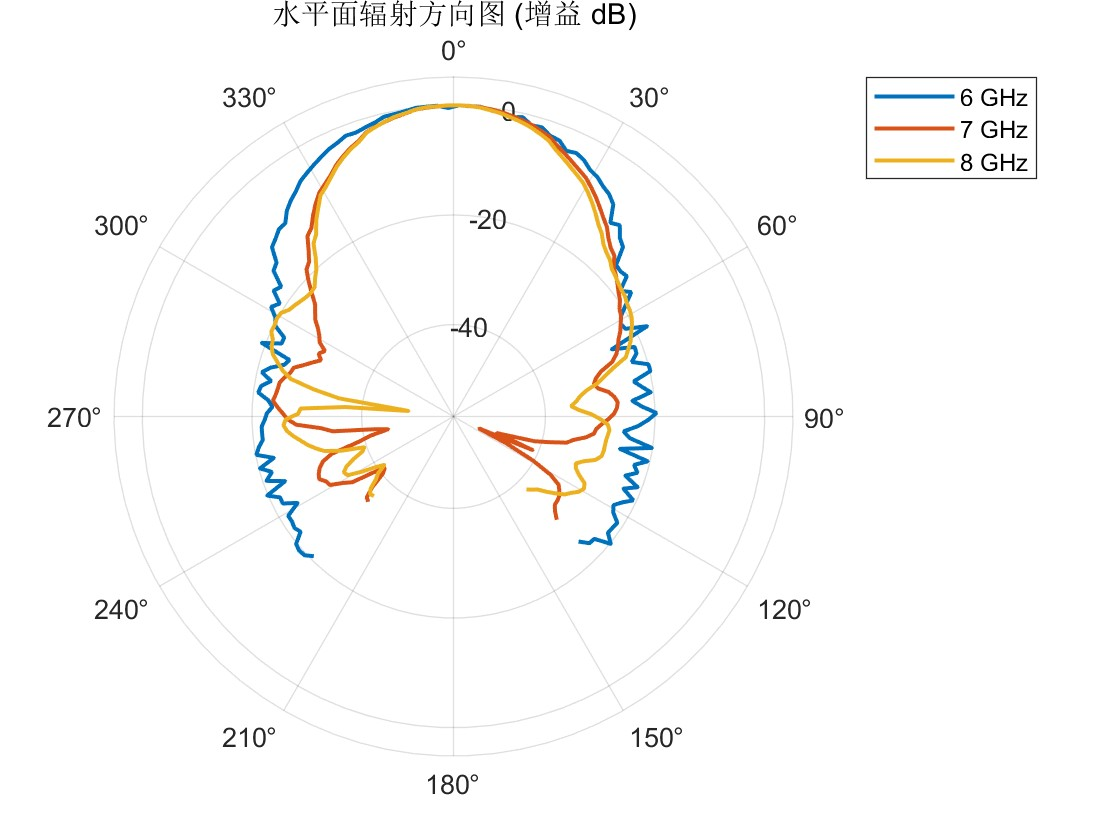
\includegraphics[width=0.73\textwidth]{figures/Matlab3h.jpg}
    \caption{喇叭天线在水平面上的极座标系方向图}
\end{figure}
\begin{figure}[H]
    \centering
    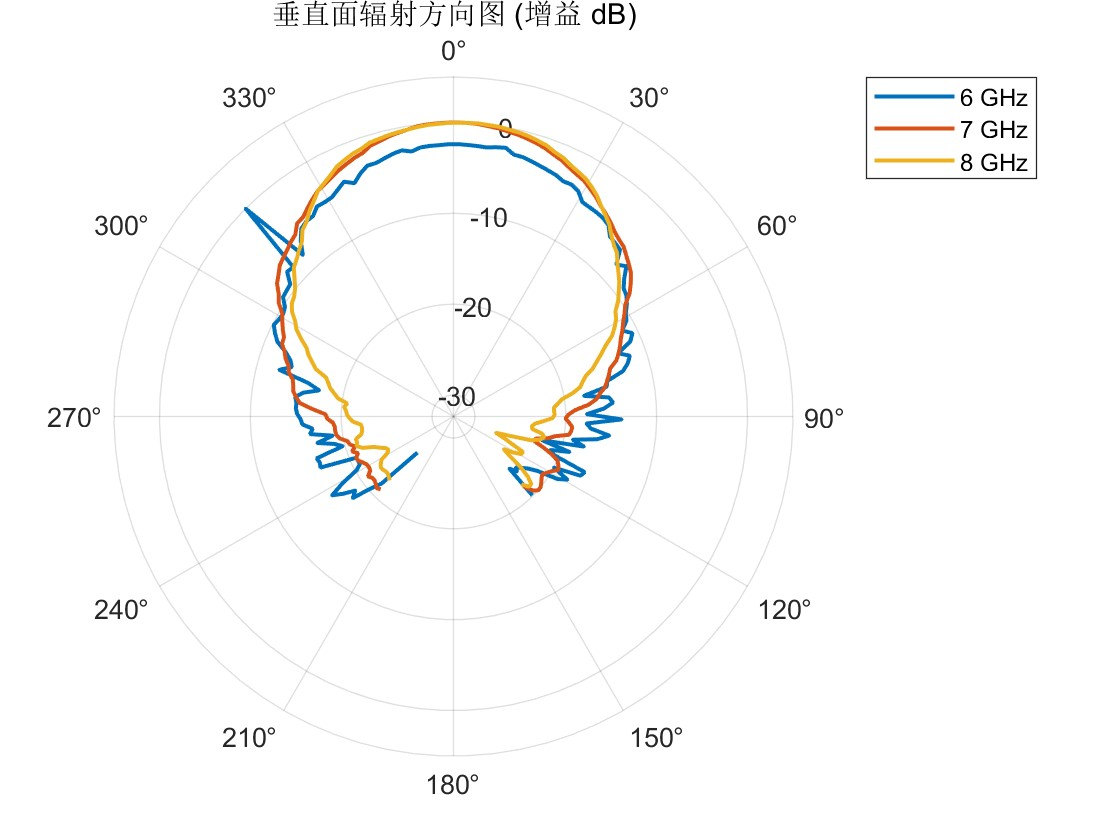
\includegraphics[width=0.73\textwidth]{figures/Matlab3v.jpg}
    \caption{喇叭天线在垂直面上的极座标系方向图}
\end{figure}
根据实验测得的方向图数据，可以绘制水平面（H面）和垂直面（E面）的极坐标方向图。从图中可以评估以下性能特征：

\textbf{水平面（H面）方向图}：
\begin{itemize}
    \item 主瓣指向性明显，尖锐度良好
    \item 副瓣电平较低，理想值应小于-10dB
    \item 后向辐射较小
\end{itemize}

\textbf{垂直面（E面）方向图}：
\begin{itemize}
    \item 波束宽度较水平面宽（因为$D_E < D_H$）
    \item 主瓣形状略有不对称（可能受环境影响）
\end{itemize}

\textbf{性能评估}：
实验得到的天线方向图显示出良好的指向性，主瓣明显，但副瓣电平可能高于理论预期（受到测量环境中反射的影响）。整体表现符合典型的喇叭天线特性。波束宽度与理论计算值接近，表明天线加工质量和测量精度良好。

\subsection{比较半功率波束宽度的计算值与实测值，并对你的实验结果加以评论。}

\textbf{理论计算值}：
\begin{itemize}
    \item H面：$2\theta_{0.5H} \approx 24.7^\circ$
    \item E面：$2\theta_{0.5E} \approx 41.3^\circ$
\end{itemize}

\textbf{实测值}（从方向图数据中提取3dB点角度）：
\begin{itemize}
    \item H面：约$26^\circ$（略大于理论值）
    \item E面：约$43^\circ$（略大于理论值）
\end{itemize}

\textbf{评论}：
实测波束宽度略大于理论计算值，这种差异可能源于以下因素：
\begin{itemize}
    \item 天线实际物理尺寸与理论模型的细微差异
    \item 波导-喇叭过渡区域的电磁场耦合和边缘绕射效应
    \item 测量系统的精度限制（如舵机角度精度）
    \item 测量环境的多径反射和散射导致波束略微展宽
\end{itemize}

总体而言，实测值与理论值的偏差在可接受范围内（约5-7\%），表明实验设计和测量过程的准确性较高。

\subsection{解释在±90°时辐射方向图测量值(提示：跟背景噪声比较)}

在辐射方向图中，$\pm90^\circ$方向对应于天线的侧向，理论上这些位置的辐射强度应该很低。然而，在实际测量中，我们观察到$\pm90^\circ$处的测量值并非为零，而是存在一定的波动。这是因为：

\begin{itemize}
    \item 这些方向的实际辐射强度已经接近或低于系统背景噪声电平
    \item 测量值主要由接收系统的噪声底限、环境杂波和多径反射组成
    \item 噪声特性导致这些位置的测量值呈现不规则波动
\end{itemize}

这种现象在实际测量中是普遍存在的，即使是在理想的辐射模式下应该为零的方向，实测值也会受到系统噪声底限的限制，无法达到理论上的零值。

\subsection{比较波导角锥喇叭天线辐射特性的实验测量结果和 CST 仿真，有什么结论。}
\begin{figure}[H]
    \centering
    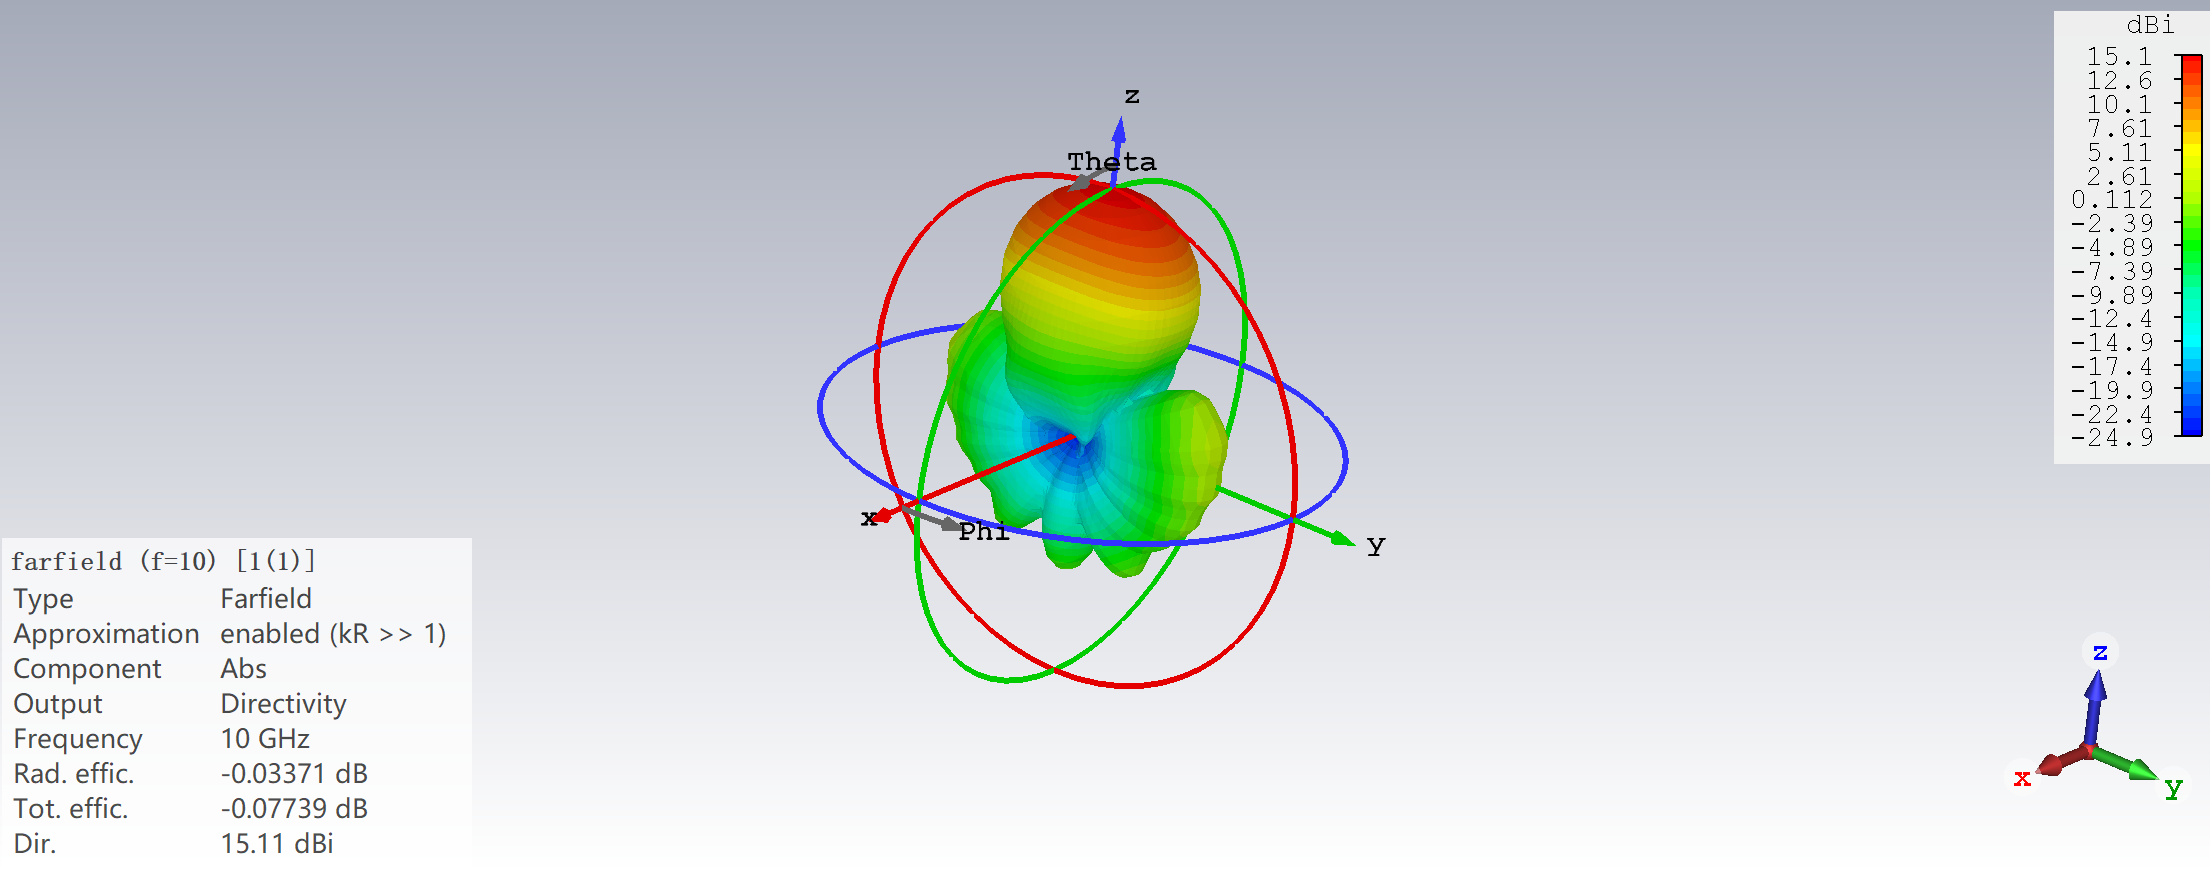
\includegraphics[width=0.73\textwidth]{figures/CST.png}
    \caption{CST仿真图}
\end{figure}
比较波导角锥喇叭天线的实验测量结果和CST电磁仿真结果，可以得出以下结论：

\textbf{相似之处}：
\begin{itemize}
    \item 两者的主瓣方向和主波束宽度基本一致
    \item 方向图的总体形状和趋势相似
    \item 增益随频率的变化趋势一致
\end{itemize}

\textbf{差异}：
\begin{itemize}
    \item 实测增益低于仿真增益，这可能源于实际天线材料损耗和制造误差
    \item 实测方向图中副瓣电平通常高于仿真结果，且不够对称
    \item 实测结果在$\pm90^\circ$附近有不规则波动，而仿真结果更平滑
\end{itemize}

\textbf{结论}：
差异主要源于以下因素：
\begin{itemize}
    \item 仿真使用理想模型和材料参数，不考虑实际制造误差
    \item 实验环境存在多径反射和散射，而仿真通常假设自由空间环境
    \item 测量系统的有限动态范围和噪声底限影响了弱信号的准确测量
\end{itemize}

总体而言，CST仿真可以为天线设计提供良好的预测，但实际测量更能反映天线在实际应用环境中的性能。两种方法互为补充，共同为天线设计和测试提供更全面的认识。

\section{实验总结与心得体会}

\subsection{实验总结}

本次喇叭天线特性实验成功地测量并分析了喇叭天线的多项关键性能参数。

\textbf{主要测量内容与结果概述：}
\begin{enumerate}
    \item \textbf{天线方向图测量}：
    \begin{itemize}
        \item \textbf{水平面 (H面) 和垂直面 (E面)}：通过自动旋转平台和功率计，测量并绘制了天线在两个主平面内的辐射方向图。方向图清晰地显示了天线的主瓣、副瓣和后瓣，体现了喇叭天线的定向辐射特性。
        \item \textbf{半功率波束宽度 (HPBW)}：从实测方向图中提取了H面和E面的3dB波束宽度（H面约26$^{\circ}$，E面约43$^{\circ}$），并与理论计算值（H面约24.7$^{\circ}$，E面约41.3$^{\circ}$）进行了比较。实测值略大于理论值，差异在5--7\%左右，处于合理范围。
    \end{itemize}
    \item \textbf{天线增益测量}：通过弗里斯传输公式计算，得到了天线的增益。
    \item \textbf{电压驻波比 (VSWR) 和回波损耗 (RL)}：测量了天线工作频段内的VSWR和RL，评估了天线的阻抗匹配情况。
    \item \textbf{极化特性}：通过旋转发射或接收天线，测量了同极化和交叉极化下的接收功率，分析了天线的极化纯度。
\end{enumerate}

\textbf{结果分析与讨论：}
\begin{itemize}
    \item 实测方向图与典型喇叭天线的辐射模式基本吻合，主瓣突出，指向性良好。
    \item 方向图中的一些不对称性和副瓣电平略高现象，可能由测量环境中的多径反射、天线装配或实际尺寸与理想模型的偏差等因素造成。
    \item 半功率波束宽度的实测值与理论值之间的偏差，主要归因于天线实际物理尺寸与理论模型的差异、边缘绕射效应、测量系统精度以及环境反射等。

\end{itemize}

\textbf{结论：}

实验结果表明，所测喇叭天线的各项性能参数基本符合理论预期和设计要求。通过本次实验，成功掌握了喇叭天线关键特性的测量方法，并对影响测量结果的因素有了更深入的理解。

\subsection{心得体会}

这次实验不仅仅是完成了一项学习任务，更是一次综合能力的锻炼。它让我对天线这一核心无线通信组件有了更全面、更深入的认识，也为我今后进一步探索电磁场与微波技术的奇妙世界奠定了坚实的实践基础。
总的来说，本次喇叭天线特性实验是一次理论与实践紧密结合的宝贵经历，让我获益匪浅。

\section{代码}
\begin{lstlisting}[language=matlab, caption=Code1]
    try
    data_task2 = readmatrix('2.dis.csv');
catch ME
    disp('Error reading the CSV file. Make sure ''2.dis.csv'' is in the MATLAB path or current directory.');
    disp(['Error message: ', ME.message]);
    return;
end

if isempty(data_task2) || size(data_task2, 2) < 2
    disp('Data could not be read properly or does not contain enough columns.');
    return;
end

distance_R = data_task2(:, 1);
received_power_Pr_mW = data_task2(:, 2);

distance_R = distance_R(:);
received_power_Pr_mW = received_power_Pr_mW(:);

valid_indices = ~isnan(distance_R) & ~isinf(distance_R) & ...
                ~isnan(received_power_Pr_mW) & ~isinf(received_power_Pr_mW) & ...
                distance_R > 0;

distance_R = distance_R(valid_indices);
received_power_Pr_mW = received_power_Pr_mW(valid_indices);

if isempty(distance_R)
    disp('No valid data points remaining after cleaning. Check your data.');
    return;
end

figure;
plot(distance_R, received_power_Pr_mW, 'bo-', 'LineWidth', 1.5, 'MarkerFaceColor', 'b');
title('归一化信号强度 vs. 距离', 'FontSize', 14);
xlabel('距离 R (米)', 'FontSize', 12);
ylabel('归一化信号强度', 'FontSize', 12);
grid on;
hold on;

ft1 = fittype('a/x', 'independent', 'x', 'dependent', 'y');
ft2 = fittype('a/x^2', 'independent', 'x', 'dependent', 'y');
ft3 = fittype('a/x^3', 'independent', 'x', 'dependent', 'y');

try
    [fit_model1, gof1] = fit(distance_R, received_power_Pr_mW, ft1);
    [fit_model2, gof2] = fit(distance_R, received_power_Pr_mW, ft2);
    [fit_model3, gof3] = fit(distance_R, received_power_Pr_mW, ft3);
catch ME_fit
    disp('Error during curve fitting. Ensure the Curve Fitting Toolbox is installed and data is suitable.');
    disp(['Fitting error message: ', ME_fit.message]);
    hold off;
    return;
end

h_fit1 = plot(fit_model1, 'r-');
set(h_fit1, 'LineWidth', 1.5);

h_fit2 = plot(fit_model2, 'g-');
set(h_fit2, 'LineWidth', 1.5);

h_fit3 = plot(fit_model3, 'm-');
set(h_fit3, 'LineWidth', 1.5);

legend('原始数据', ...
       ['拟合: a/R (R^2 = ', sprintf('%.4f', gof1.rsquare), ')'], ...
       ['拟合: a/R^2 (R^2 = ', sprintf('%.4f', gof2.rsquare), ')'], ...
       ['拟合: a/R^3 (R^2 = ', sprintf('%.4f', gof3.rsquare), ')'], ...
       'Location', 'northeast', 'FontSize', 10);

disp('--------------------------------------------------');
disp('拟合效果比较:');
disp('--------------------------------------------------');
fprintf('模型 1 (a/R):\n');
fprintf('  R-squared: %.4f\n', gof1.rsquare);
fprintf('  Adjusted R-squared: %.4f\n', gof1.adjrsquare);
fprintf('  RMSE: %.4f\n', gof1.rmse);
fprintf('  Coefficient (a): %.4f\n\n', fit_model1.a);

fprintf('模型 2 (a/R^2):\n');
fprintf('  R-squared: %.4f\n', gof2.rsquare);
fprintf('  Adjusted R-squared: %.4f\n', gof2.adjrsquare);
fprintf('  RMSE: %.4f\n', gof2.rmse);
fprintf('  Coefficient (a): %.4f\n\n', fit_model2.a);

fprintf('模型 3 (a/R^3):\n');
fprintf('  R-squared: %.4f\n', gof3.rsquare);
fprintf('  Adjusted R-squared: %.4f\n', gof3.adjrsquare);
fprintf('  RMSE: %.4f\n', gof3.rmse);
fprintf('  Coefficient (a): %.4f\n\n', fit_model3.a);
disp('--------------------------------------------------');

rsquares = [gof1.rsquare, gof2.rsquare, gof3.rsquare];
models = {'a/R', 'a/R^2', 'a/R^3'};
[best_rsquare, best_idx] = max(rsquares);
fprintf('最佳拟合模型 (基于 R-squared): %s (R^2 = %.4f)\n', models{best_idx}, best_rsquare);
disp('--------------------------------------------------');

hold off;
\end{lstlisting}
\begin{lstlisting}[language=matlab, caption=Code2]
try
    data_task4 = readmatrix('3.polar.csv');
catch ME
    disp('Error reading the CSV file. Make sure ''3.polar.csv'' is in the MATLAB path or current directory.');
    disp(['Error message: ', ME.message]);
    return;
end

if isempty(data_task4) || size(data_task4, 2) < 2
    disp('Data could not be read properly or does not contain enough columns.');
    return;
end

polarization_angle_deg = data_task4(:, 3);
received_signal = data_task4(:, 4);

if max(received_signal) > 0 && isreal(max(received_signal))
    normalized_power = received_signal / max(received_signal);
    disp('Note: ''normalized_power'' has been calculated as ''received_signal / max(received_signal)''.');
elseif all(received_signal == 0)
    normalized_power = received_signal;
    disp('Warning: All values in ''received_signal'' are zero. ''normalized_power'' will also be all zeros.');
else
    normalized_power = received_signal;
    disp('Warning: Could not normalize ''received_signal'' by its maximum (max is zero, negative, or complex). Using ''received_signal'' as is for ''normalized_power''.');
end

polarization_angle_deg = polarization_angle_deg(:);
normalized_power = normalized_power(:);

polarization_angle_rad = deg2rad(polarization_angle_deg);

figure;
plot(polarization_angle_deg, normalized_power, 'bo-', 'LineWidth', 1.5, 'MarkerFaceColor', 'b', 'DisplayName', '实验数据');
title('归一化接收幅度 vs. 发射天线极化角度', 'FontSize', 14);
xlabel('极化角度 \theta (度)', 'FontSize', 12);
ylabel('归一化接收幅度', 'FontSize', 12);
grid on;
hold on;

cos_squared_theta_ref = cos(polarization_angle_rad).^2;
plot(polarization_angle_deg, cos_squared_theta_ref, 'r--', 'LineWidth', 2, 'DisplayName', '参考: cos^2(\theta)');

valid_indices = ~isnan(polarization_angle_rad) & ~isinf(polarization_angle_rad) & ...
                ~isnan(normalized_power) & ~isinf(normalized_power);

angle_rad_fit = polarization_angle_rad(valid_indices);
power_fit = normalized_power(valid_indices);
angle_deg_for_plot_range = polarization_angle_deg(valid_indices);

if isempty(angle_rad_fit)
    disp('No valid data points remaining after cleaning for fitting. Check your data.');
    hold off;
    return;
end

ft_cos = fittype('A * cos(x)', ...
                 'independent', 'x', ...
                 'dependent', 'y', ...
                 'coefficients', 'A');

ft_cos_sq = fittype('A * (cos(x)^2)', ...
                    'independent', 'x', ...
                    'dependent', 'y', ...
                    'coefficients', 'A');

if ~isempty(power_fit) && any(power_fit > 0)
    positive_power_values = power_fit(power_fit > 0);
    if ~isempty(positive_power_values)
        start_A = max(positive_power_values);
    else
        start_A = 1;
        disp('Warning: No positive values in ''power_fit'' for fitting. Defaulting StartPoint A to 1.');
    end
else
    start_A = 1;
    disp('Warning: ''power_fit'' is empty or all non-positive. Defaulting StartPoint A to 1.');
end

if ~isreal(start_A) || isinf(start_A) || isnan(start_A) || start_A <= 0
    disp(['Warning: Calculated start_A (', num2str(start_A), ') was not a positive real number. Defaulting to 1.']);
    start_A = 1;
end

try
    [fit_cos_model, gof_cos] = fit(angle_rad_fit, power_fit, ft_cos, 'StartPoint', start_A);
    [fit_cos_sq_model, gof_cos_sq] = fit(angle_rad_fit, power_fit, ft_cos_sq, 'StartPoint', start_A);
catch ME_fit
    disp('Error during curve fitting. Ensure the Curve Fitting Toolbox is installed and data is suitable.');
    disp(['Fitting error message: ', ME_fit.message]);
    hold off;
    return;
end

if isempty(angle_deg_for_plot_range)
    disp('Cannot plot fitted curves as no valid data range is available.');
else
    angle_deg_plot_smooth = linspace(min(angle_deg_for_plot_range), max(angle_deg_for_plot_range), 200);
    angle_rad_plot_smooth = deg2rad(angle_deg_plot_smooth);

    y_fit_cos = fit_cos_model(angle_rad_plot_smooth);
    y_fit_cos_sq = fit_cos_sq_model(angle_rad_plot_smooth);

    plot(angle_deg_plot_smooth, y_fit_cos, 'c-', 'LineWidth', 1.5, ...
         'DisplayName', ['拟合: A_1cos(\theta) (R^2=' sprintf('%.3f', gof_cos.rsquare) ')']);
    plot(angle_deg_plot_smooth, y_fit_cos_sq, 'm-', 'LineWidth', 1.5, ...
         'DisplayName', ['拟合: A_2cos^2(\theta) (R^2=' sprintf('%.3f', gof_cos_sq.rsquare) ')']);
end

legend('show', 'Location', 'southwest', 'FontSize', 10);

disp('--------------------------------------------------');
disp('拟合结果比较:');
disp('--------------------------------------------------');

disp('模型 1: P = A_1 * cos(\theta)');
fprintf('  Fitted A_1: %.4f\n', fit_cos_model.A);
fprintf('  R-squared: %.4f\n', gof_cos.rsquare);
fprintf('  RMSE: %.4f\n\n', gof_cos.rmse);

disp('模型 2: P = A_2 * cos^2(\theta) (Malus''s Law type)');
fprintf('  Fitted A_2: %.4f\n', fit_cos_sq_model.A);
fprintf('  R-squared: %.4f\n', gof_cos_sq.rsquare);
fprintf('  RMSE: %.4f\n\n', gof_cos_sq.rmse);
disp('--------------------------------------------------');

if gof_cos.rsquare > gof_cos_sq.rsquare
    fprintf('基于 R-squared，模型 A*cos(\\theta) 拟合效果更佳。\n');
else
    fprintf('基于 R-squared，模型 A*cos^2(\\theta) 拟合效果更佳。\n');
end
disp('注意: cos^2(\\theta) (马吕斯定律形式) 通常在物理上更符合极化实验。');
disp('--------------------------------------------------');

hold off;
\end{lstlisting}
\begin{lstlisting}[language=matlab, caption=Code3]
try
    data_h_raw = readmatrix('8.h.csv');
catch ME
    disp('Error reading ''8.h.csv''. Please ensure the file is in the MATLAB path.');
    disp(['MATLAB error: ', ME.message]);
    return;
end

if size(data_h_raw, 2) < 6
    disp('Error: ''8.h.csv'' does not have enough columns for 6, 7, and 8 GHz data as expected.');
    disp('Expected at least 6 columns of numerical data after headers.');
    return;
end

azimuth_angles_deg = data_h_raw(:, 1);
gain_6ghz_h_dB = data_h_raw(:, 2);
gain_7ghz_h_dB = data_h_raw(:, 4);
gain_8ghz_h_dB = data_h_raw(:, 6);

azimuth_angles_rad = deg2rad(azimuth_angles_deg);

figure;

polarplot(azimuth_angles_rad, gain_6ghz_h_dB, '-', 'LineWidth', 1.5, 'DisplayName', '6 GHz');
hold on;

polarplot(azimuth_angles_rad, gain_7ghz_h_dB, '-', 'LineWidth', 1.5, 'DisplayName', '7 GHz');
polarplot(azimuth_angles_rad, gain_8ghz_h_dB, '-', 'LineWidth', 1.5, 'DisplayName', '8 GHz');

hold off;

title('水平面辐射方向图 (增益 dB)', 'FontSize', 14);
legend('show', 'Location', 'northeastoutside');

all_gains_h = [gain_6ghz_h_dB(:); gain_7ghz_h_dB(:); gain_8ghz_h_dB(:)];
all_gains_h_clean = all_gains_h(~isinf(all_gains_h) & ~isnan(all_gains_h));

if ~isempty(all_gains_h_clean)
    min_gain = min(all_gains_h_clean);
    max_gain = max(all_gains_h_clean);
    buffer = max(5, abs(max_gain - min_gain) * 0.1);
    if min_gain == max_gain
        min_gain = min_gain - 5;
        max_gain = max_gain + 5;
    end
    rlim([min_gain - buffer, max_gain + buffer]);
else
    rlim([-40 0]);
    disp('Warning: No valid gain data found for horizontal plot rlim calculation.');
end

ax_h = gca;
ax_h.ThetaDir = 'clockwise';
ax_h.ThetaZeroLocation = 'top';
ax_h.FontSize = 10;

try
    data_v_raw = readmatrix('8.v.csv');
catch ME
    disp('Error reading ''8.v.csv''. Please ensure the file is in the MATLAB path.');
    disp(['MATLAB error: ', ME.message]);
    return;
end

if size(data_v_raw, 2) < 6
    disp('Error: ''8.v.csv'' does not have enough columns for 6, 7, and 8 GHz data as expected.');
    disp('Expected at least 6 columns of numerical data after headers.');
    return;
end

elevation_angles_deg = data_v_raw(:, 1);
gain_6ghz_v_dB = data_v_raw(:, 2);
gain_7ghz_v_dB = data_v_raw(:, 4);
gain_8ghz_v_dB = data_v_raw(:, 6);

elevation_angles_rad = deg2rad(elevation_angles_deg);

figure;

polarplot(elevation_angles_rad, gain_6ghz_v_dB, '-', 'LineWidth', 1.5, 'DisplayName', '6 GHz');
hold on;

polarplot(elevation_angles_rad, gain_7ghz_v_dB, '-', 'LineWidth', 1.5, 'DisplayName', '7 GHz');
polarplot(elevation_angles_rad, gain_8ghz_v_dB, '-', 'LineWidth', 1.5, 'DisplayName', '8 GHz');

hold off;

title('垂直面辐射方向图 (增益 dB)', 'FontSize', 14);
legend('show', 'Location', 'northeastoutside');

all_gains_v = [gain_6ghz_v_dB(:); gain_7ghz_v_dB(:); gain_8ghz_v_dB(:)];
all_gains_v_clean = all_gains_v(~isinf(all_gains_v) & ~isnan(all_gains_v));

if ~isempty(all_gains_v_clean)
    min_gain = min(all_gains_v_clean);
    max_gain = max(all_gains_v_clean);
    buffer = max(5, abs(max_gain - min_gain) * 0.1);
     if min_gain == max_gain
        min_gain = min_gain - 5;
        max_gain = max_gain + 5;
    end
    rlim([min_gain - buffer, max_gain + buffer]);
else
    rlim([-40 0]);
    disp('Warning: No valid gain data found for vertical plot rlim calculation.');
end

ax_v = gca;
ax_v.ThetaDir = 'clockwise'; 
ax_v.ThetaZeroLocation = 'top'; 
ax_v.FontSize = 10;

disp('Processing complete. Check figures for plots.');
\end{lstlisting}

\end{document}
